% define documentclass
\documentclass[12pt, bibliography=totoc, a4paper, abstractoff, numbers=noenddot]{scrreprt}
\setcounter{secnumdepth}{3} 

% define used packages
\usepackage[left=4.0cm, right=2.0cm, top=3cm, bottom=3cm]{geometry}
%\usepackage{bibgerm}
\usepackage{babelbib}
\usepackage[utf8]{inputenc}
\usepackage[T1]{fontenc}
\usepackage{graphicx}
\usepackage[ngerman]{babel}
\usepackage{lmodern}
\usepackage{listings}
\usepackage[numbers]{natbib}
\usepackage{acronym}
\bibliographystyle{alphadin}
\usepackage{float}
\usepackage[title]{appendix}
\usepackage[table,xcdraw]{xcolor}
\usepackage{tabularx}
\usepackage{multirow}

\usepackage{lastpage}

% advanced tables
\usepackage{array}

% header and footer
\usepackage{fancyhdr}

% links
\usepackage{url}
% internal links
\usepackage[colorlinks=true ,linkcolor=black,
			anchorcolor=black ,citecolor=black ,filecolor=black,
			menucolor=black ,urlcolor=black]{hyperref}

%Makroerweiterung da urls sonst über den Rand gehen
\makeatletter 
\g@addto@macro\UrlBreaks{\do\a\do\b\do\c\do\d\do\e\do\f\do\g\do\h\do\i% 
\do\j\do\k\do\l\do\m\do\n\do\o\do\p\do\q\do\r\do\s\do\t\do\u\do\v\do\w% 
\do\x\do\y\do\z\do\&\do\1\do\2\do\3\do\4\do\5\do\6\do\7\do\8\do\9\do\0} 
\def\do@url@hyp{\do\-} 
 \g@addto@macro\UrlSpecials{\do\/{\mbox{\UrlFont/}\hskip 0pt plus 1pt}}
\makeatother
% mathematical formulas
\usepackage{amsmath, amssymb}

% fancy Diagrams %
\usepackage{tikz}
\usepackage{epstopdf}

% to include images side by side
\usepackage{subfigure}

% for nice bg on title page
\usepackage{eso-pic}
\newcommand\BackgroundPic{%
\put(0,0){%
\parbox[b][\paperheight]{\paperwidth}{%
\vfill
\centering
\includegraphics[width=\paperwidth,height=\paperheight,%
keepaspectratio]{images/Logo_H-BRS_background}%
\vfill
}}}

% define the programming language
\input{lststyles}

%set default pagestyle
\pagestyle{empty}


\setlength{\parindent}{0pt}
\setlength{\parskip}{12pt}

% #####
% #
% # START config area
% #
% #####

\newcommand{\HEADER}[0]{H-BRS, WS 2016 / 2017}
\newcommand{\PAGENUMBERS}[0]{\pagemark}
\newcommand{\DATE}[0]{12.10.2016}
\newcommand{\AUTHOR}[0]{Eugen Besel, Johann Martens, Moritz Kemp}
\newcommand{\MATNR}[0]{}
\newcommand{\STREET}[0]{}
\newcommand{\ZIP}[0]{}
\newcommand{\TOWN}[0]{}

\newcommand{\REFERENT}[0]{Prof. Dr. Harm Knolle}
%\newcommand{\KOREFERENT}[0]{}

\newcommand{\TITLE}[0]{Aufbau einer NoSQL-Datenbank mit Apache Hadoop und Apache HBase für das Million Song Dataset}
\newcommand{\COURSE}[0]{Schemalose Datenbanken}
\newcommand{\TYPE}[0]{Semester-Projekt}
\newcommand{\COMPLETION}[0]{}

% #####
% #
% # END config area
% #
% #####

% Hurenkinder und Schusterjungenregelung
\clubpenalty=100000
\widowpenalty=100000
\displaywidowpenalty=100000

%TODO: auf Fragezeichen überprüfen
% starting the document
\begin{document}

% set pagenumbering to roman(I II III IV)
\pagenumbering{Roman}
% input the title
\input{title}
%Zusammenfassung
\begin{abstract}
\section*{Zusammenfassung}\markboth{Zusammenfassung}{}
  \addcontentsline{toc}{chapter}{Zusammenfassung}
  Das Ziel der Projektarbeit zum Thema \textit{Hadoop/Hbase} ist es, 
eine Datenbank mittels Hadoop/Hbase auf einem bereitgestelltem
Cluster so zu installieren, dass der Anwender in dem One-Million-Datensatz nach Informationen zu Musikstücken
suchen kann. 

%Im ersten Teil der Projektarbeit werden die theoretischen Grundlagen von Hadoop/Hbase 
%behandelt. Dieser Teil beinhaltet ein Kapitel zu Map/Reduce, ein Kapitel zu Hadoop und ein Kapitel zu Hbase.
%Die Theorie soll etwa ein Drittel der Projektarbeit ausmachen. 

Im ersten Teil der Projektarbeit werden die technologischen Grundlagen zu MapReduce
behandelt.Die Theorie soll etwa ein Drittel der Projektarbeit ausmachen. Im zweiten Kapitel werden das NoSQL-System HBase und Hadoop vorgestellt.
Hier wird auch Schritt für Schritt das Vorgehen  beschrieben, wie die Installation und Konfiguration 
der Systeme abläuft. Fragestellungen werden sein, wie 
sich die Datenbank auf einen Cluster installieren lässt und welche Konfigurationsparameter hinsichtlich des
Anwendungsfalls eines One-Million-Datensatzes berücksichtigt und angepasst werden müssen.

Der dritte Teil der Projektarbeit beschreibt die praktische Umsetzung, die aus der Implementierung der Client-Software besteht.
Eingangs werden Anforderungen, Anwendungsfälle und technische Rahmenbedingungen kurz beschrieben,
um einen Überblick zu geben.   %Eingesetzte Programmiersprache ist hier Java.
Auch die konkrete
Implementierung des MapReduce-Algorithmus wird in diesem Kapitel dargelegt. Des Weiteren werden Filter- und Optimierungsparameter,
die besonders HBase betreffen, evaluiert und gegebenenfalls angewendet.

Außerdem wird gezeigt,
ob und wie sich die Datenbank auch ohne eigens programmiertem Client Ad-Hoc ansprechen lässt, beispielsweise über
eine laufende Shell. Das nächste Kapitel beschreibt die Implementierung der Client-Software, die mittels Java als Serveranwendung
und Java als Client-Anwendung dem Anwender die Möglichkeit bieten soll, über eine grafische Oberfläche mit dem One-Million-Datensatz zu arbeiten. Der Client beschränkt sich dabei auf wenige, nur funktionale Anforderungen. Eine aufwendig grafische Oberfläche ist nicht das Ziel.
Ein weiteres Kapitel im praktischen Teil behandelt die Installation des One-Million-Song-Datensatzes in das Hadoop-Dateisystem.
Wichtige Fragestellungen sind dabei, inwieweit die Daten bereits für die Speicherung im Hadoop-Dateisystem geeignet sind und
die Frage nach der Replikation auf dem Cluster-System.

Zum Abschluss des praktischen Teils folgt eine kurze Leistungsdarstellung des Systems, indem die Antwortzeiten
der Datenbank zu bestimmten Abfragen gemessen werde. Optional ist eine Leistungsbewertung im Vergleich mit 
einem anderen Team denkbar, die ebenfalls mit dem selben Datensatz arbeiten.


%Das Team wird sich zuerst mit den Grundlagen von NoSQL-Datenbanken befassen, 
%vor allem explizit mit den Grundlagen von Hadoop/Hbase. Darauf aufbauend lässt
%sich eine Argumentation formulieren, warum sich die Behandlung von derart großen Datensätzen
%wie dem Million-Song-Datensatz mit Hadoop/Hbase effektiver gestalten lässt als mit klassischen relationalen Datenbanken. Dieser Teil beinhaltet also im wesentlichen
%Grundlagen zu den Wide-Column-Datenbanken sowie Grundlagen zu Hadoop und Hbase.

%Im praktischen Teil wird zunächst die benötigte Software installiert, i.e. Java, Hadoop und HBase. Um die Installation auf einer Windows-Maschine auszuführen wird zusätzlich Cygwin installiert. Um auf die HBase-Datenbank zugreifen zu können, muss HBase zunächst konfiguriert werden.

%Nach erfolgreicher Installation wird HBASE zunächst im Standalone-Modus auf einer Maschine betrieben. Zur Anschauung wird eine Tabelle angelegt und es werden CRUD-Operationen geschildert. Im Anschluss daran wird gezeigt, wie man programmatisch mit der Datenbank arbeiten kann mit Hilfe von JRuby.

%Nach den ersten Tests wird der Import von Daten (One-Million-Song-Datensatz) beschrieben und durchgeführt. Für die Verwaltung der Daten wird eine Client-Anwendung mit Ruby geschrieben.

%Im letzten Schritt wird HBase auf dem Hochschul-Cluster installiert und für den Cluster-Modus konfiguriert.

%\begin{itemize}
%\item[28.10] - Expose
%\item[25.11] - HBase im Standalone-Modus auf einer Windows-Maschine installieren und CRUD-Operationen mit Testdaten durchführen.
%\item[25.11] - One-Million-Dataset importieren
%\item[02.12] - Zwischenbericht
%\item[02.12] - MapReduce-Kapitel 6C
%\item[02.12] - Hadoop-Kapitel 6D1  
%\item[16.12] - HBase-Kapitel 6D2 
%\item[16.12] - Client-Anwendung fertig stellen
%\item[23.12] - Cluster-Installation abgeschlossen
%\item[06.01] - Ausarbeitung Projektarbeit
%\end{itemize}

\end{abstract}


% Vorwort -TODO:Darf nicht  nicht im semesterergebnis erscheinen
% \renewcommand\abstractname{Danksagung}
\begin{abstract}
\section*{Vorwort}\markboth{Vorwort}{}
  \addcontentsline{toc}{chapter}{Vorwort}
  
% Please add the following required packages to your document preamble:
% \usepackage{graphicx}
% \usepackage[table,xcdraw]{xcolor}
% If you use beamer only pass "xcolor=table" option, i.e. \documentclass[xcolor=table]{beamer}
\begin{table}[ht!]
\centering
\resizebox{\textwidth}{!}{%
\begin{tabular}{|l|l|l|l|l|}
\hline
\rowcolor[HTML]{EFEFEF} 
Thema                                                                                                                                  & \begin{tabular}[c]{@{}l@{}}Hauptverantwortlicher\\ schriftliche Ausarbeitung\end{tabular} & \begin{tabular}[c]{@{}l@{}}Hauptverantwortlicher \\ praktische Umsetzung am Rechner\end{tabular} & \begin{tabular}[c]{@{}l@{}}Hauptverantwortlicher \\ Erstellung Vortrag\end{tabular} & \begin{tabular}[c]{@{}l@{}}Hauptverantwortlicher \\ Vortrag vorgetragen\end{tabular} \\ \hline
\begin{tabular}[c]{@{}l@{}}Ausgewählte\\ technologische Grundlagen\end{tabular}                                                        & Moritz                                                                                    & Moritz                                                                                           & Moritz                                                                              & Moritz                                                                               \\ \hline
\begin{tabular}[c]{@{}l@{}}Ausgewählte Persistenzsysteme \\ und Big Data Frameworks\\ - Vorstellung des Systems\end{tabular}           & \begin{tabular}[c]{@{}l@{}}Hadoop: Eugen\\ HBase: Johann\end{tabular}                     & -                                                                                                & Johann                                                                              & \begin{tabular}[c]{@{}l@{}}Hadoop: Eugen\\ HBase: Johann\end{tabular}                \\ \hline
\begin{tabular}[c]{@{}l@{}}Ausgewählte Persistenzsysteme \\ und Big Data Frameworks\\ - Installation des Systems\end{tabular}          & \begin{tabular}[c]{@{}l@{}}Hadoop: Moritz\\ HBase: Johann\end{tabular}                    & \begin{tabular}[c]{@{}l@{}}Hadoop: Moritz\\ HBase: Johann\end{tabular}                           & Moritz                                                                              & Moritz                                                                               \\ \hline
\begin{tabular}[c]{@{}l@{}}Ausgewählte Persistenzsysteme \\ und Big Data Frameworks\\ - Ad-Hoc-Anwendungen \\ des Systems\end{tabular} & Johann                                                                                    & Eugen                                                                                            & Johann                                                                              & Johann                                                                               \\ \hline
\begin{tabular}[c]{@{}l@{}}Ausgewählte Persistenzsysteme \\ -Implementierung der \\ Beispiel-Datenbank\end{tabular}                    & Eugen                                                                                     & Eugen                                                                                            & Johann                                                                              & Johann                                                                               \\ \hline
\begin{tabular}[c]{@{}l@{}}Ausgewählte Anwendungsszenarien\\ - Spezifikation des \\ Anwendungsszenarios\end{tabular}                   & Johann                                                                                    & \begin{tabular}[c]{@{}l@{}}HBase: Eugen\\ MapReduce-Jobs: Moritz\end{tabular}                    & Johann                                                                              & Johann                                                                               \\ \hline
\begin{tabular}[c]{@{}l@{}}Ausgewählte Anwendungsszenarien\\ - Spezifikation der konkreten \\ Anwendung\end{tabular}                   & Eugen                                                                                  & \begin{tabular}[c]{@{}l@{}}HBase: Eugen\\ MapReduce-Jobs: Moritz\end{tabular}                    & Eugen                                                                               & Eugen                                                                                \\ \hline
\begin{tabular}[c]{@{}l@{}}Ausgewählte Anwendungsszenarien\\ - Implementierung der Anwendung\end{tabular}                              & Eugen                                                                                     & \begin{tabular}[c]{@{}l@{}}HBase: Eugen\\ MapReduce-Jobs: Moritz\end{tabular}                    & Johann                                                                              & Eugen                                                                                \\ \hline
\end{tabular}%
}
\caption{Zuständigkeiten im Laufe des Semesterprojekts}
\label{my-label}
\end{table}
\end{abstract}


%Inhaltsverzeichnis
% loads the fancy pagestyle for register part
\input{fancyRegisterPart}

% create the registers
\tableofcontents\newpage

% set pagenumbering to arabic(1 2 3 4)
\pagenumbering{arabic}
% loads the fancy pagestyle for main part
\input{fancyMainPart}



% #####
% # load the chapter from the files
% #
% # TODO: create new chapter
% #####
\chapter{Ausgewählte technologische Grundlagen}
\section{Das MapReduce-Framework}
MapReduce wurde 2004 von zwei Mitarbeitern von Google vorgestellt \cite{dean2008mapreduce}. Es ist ein Framework
für die Entwicklung von massiver, paralleler Datenverarbeitung sehr großen Datenmengen auf Clustern.



Der Programmierer
kann sich dabei komplett auf die Verarbeitung der Daten konzentrieren. Das Framework kümmert sich um die parallele
Ausführung der Arbeit, ohne dass der Programmierer der Anwendung wissen muss, welche Daten konkret wo verteilt vorliegen
und verarbeitet werden. 
Im Zusammenarbeit mit speziellen Filesystemen 
für große Cluster-Systeme, die zum Beispiel automatisch redundante Kopien auf mehreren Maschinen anlegen, ermöglicht
eine mit MapReduce programmierte Anwendung zudem eine hohe Toleranz gegenüber dem Ausfall von einzelnen Maschinen.

\subsection{Arbeitsweise von MapReduce}
Auf der obersten Abstraktionsebene besteht das MapReduce-Framework nur aus zwei spezifizierten Funktionen: \textit{map} und \textit{reduce}.
Beide Funktionen müssen vom Anwender des MapReduce-Frameworks implementiert werden.
\textit{map} nimmt eine, möglicherweise ungeordnete, Liste von Daten entgegen, die Schlüssel-Wert-Paare (key/value) enthält. Die Funktion 
verarbeitet nun diese Liste nach dem vom Programmierer implementierten Funktion und liefert als Ergebnis wiederum eine
Liste von Schlüssel-Wert-Paaren. Die konkrete Logik der \textit{map}-Funktion ist vom Anwendungsfall abhängig, bildet aber in der Regel
ungeordneten Daten in eine Liste ab, die die für den Anwendungsfall interessanten Daten enthält. 


%Beispiel?
%Ein gern genommenes Beispiel
%ist das Zählen von Wörtern in tausenden von Dokumenten. Die Liste für die Eingabe in die \textit{map}-Funktion enthält für jeden Schlüssel
%als Wert ein ganzes Dokument. Diese Dokumente werden durchsucht und gleichzeitig eine neue, deutlich größere Liste mit Schlüssel-Wert-Paaren erstellt, 
%die für jedes einzelne Wort den String selbst als Schlüssel speichert, und als Wert eine 1 angibt. Somit ist jedes Wort in dieser Liste repräsentiert.
%Diese neue Liste enthält sehr viele gleiche Schlüssel, wobei alle den Wert 1 tragen.

Das Ergebnis von der \textit{map}-Funktion ist aber nur ein Zwischen-Ergebnis und wird direkt als Eingabe für die \textit{reduce}-Funktion verwendet,
die am Ende das tatsächliche Ergebnis der Verarbeitung ausgibt. Die \textit{reduce}-Funktion hat in der Regel die Aufgabe, das Ergebnis der \textit{map}-Funktion
zusammenzufassen.  

%Bezogen auf das Beispiel mit der Zählung von Wörtern bekommt die \textit{reduce}-Funktion nun eine (sehr lange) Liste von allen Wortvorkommnissen.
%Die Funktion sortiert  nun diese Liste und erzeugt eine neue Liste, die alle Schlüssel-Werte enthält, aber nur ein einziges mal in der Liste. Mehrfache Einträge
%in der ursprünglichen Liste mit gleichen Schlüsselwerten werden also zu einem Eintrag zusammengefasst, wobei die Werte der einzelne, mehrfachen Einträge
%aufaddiert werden. Das Ergebnis ist eine Liste mit jedem Wort, das in den Dokumenten vorkommt, als einmaliger Schlüssel und als Wert die jeweilige Häufigkeit.

Neben den beiden Funktionen map und reduce liefert das MapReuce-Framework auch eine Laufzeitumgebung mit, in der jene beiden Funktionen eingebettet sind.
Die Laufzeitumgebung kümmert sich dabei um die Verteilung der Arbeit auf dem Cluster. 
Dafür werden erstens die implementierten Map und Reduce-Funktionen
kopiert und auf die einzelnen Maschinen im Cluster verteilt. Zweitens werden die Eingabedaten zerteilt und die einzelnen Daten-Stücke auf die Maschinen verteilt. 

Die konkrete Implementierung der Laufzeitumgebung hängt vom Einsatzort und Zweck ab. 
Google schlägt in seinem Paper folgendes Konstrukt vor, das in Abbildung \ref{fig:mapreduce} visualisiert wird.

\begin{figure}
\centering
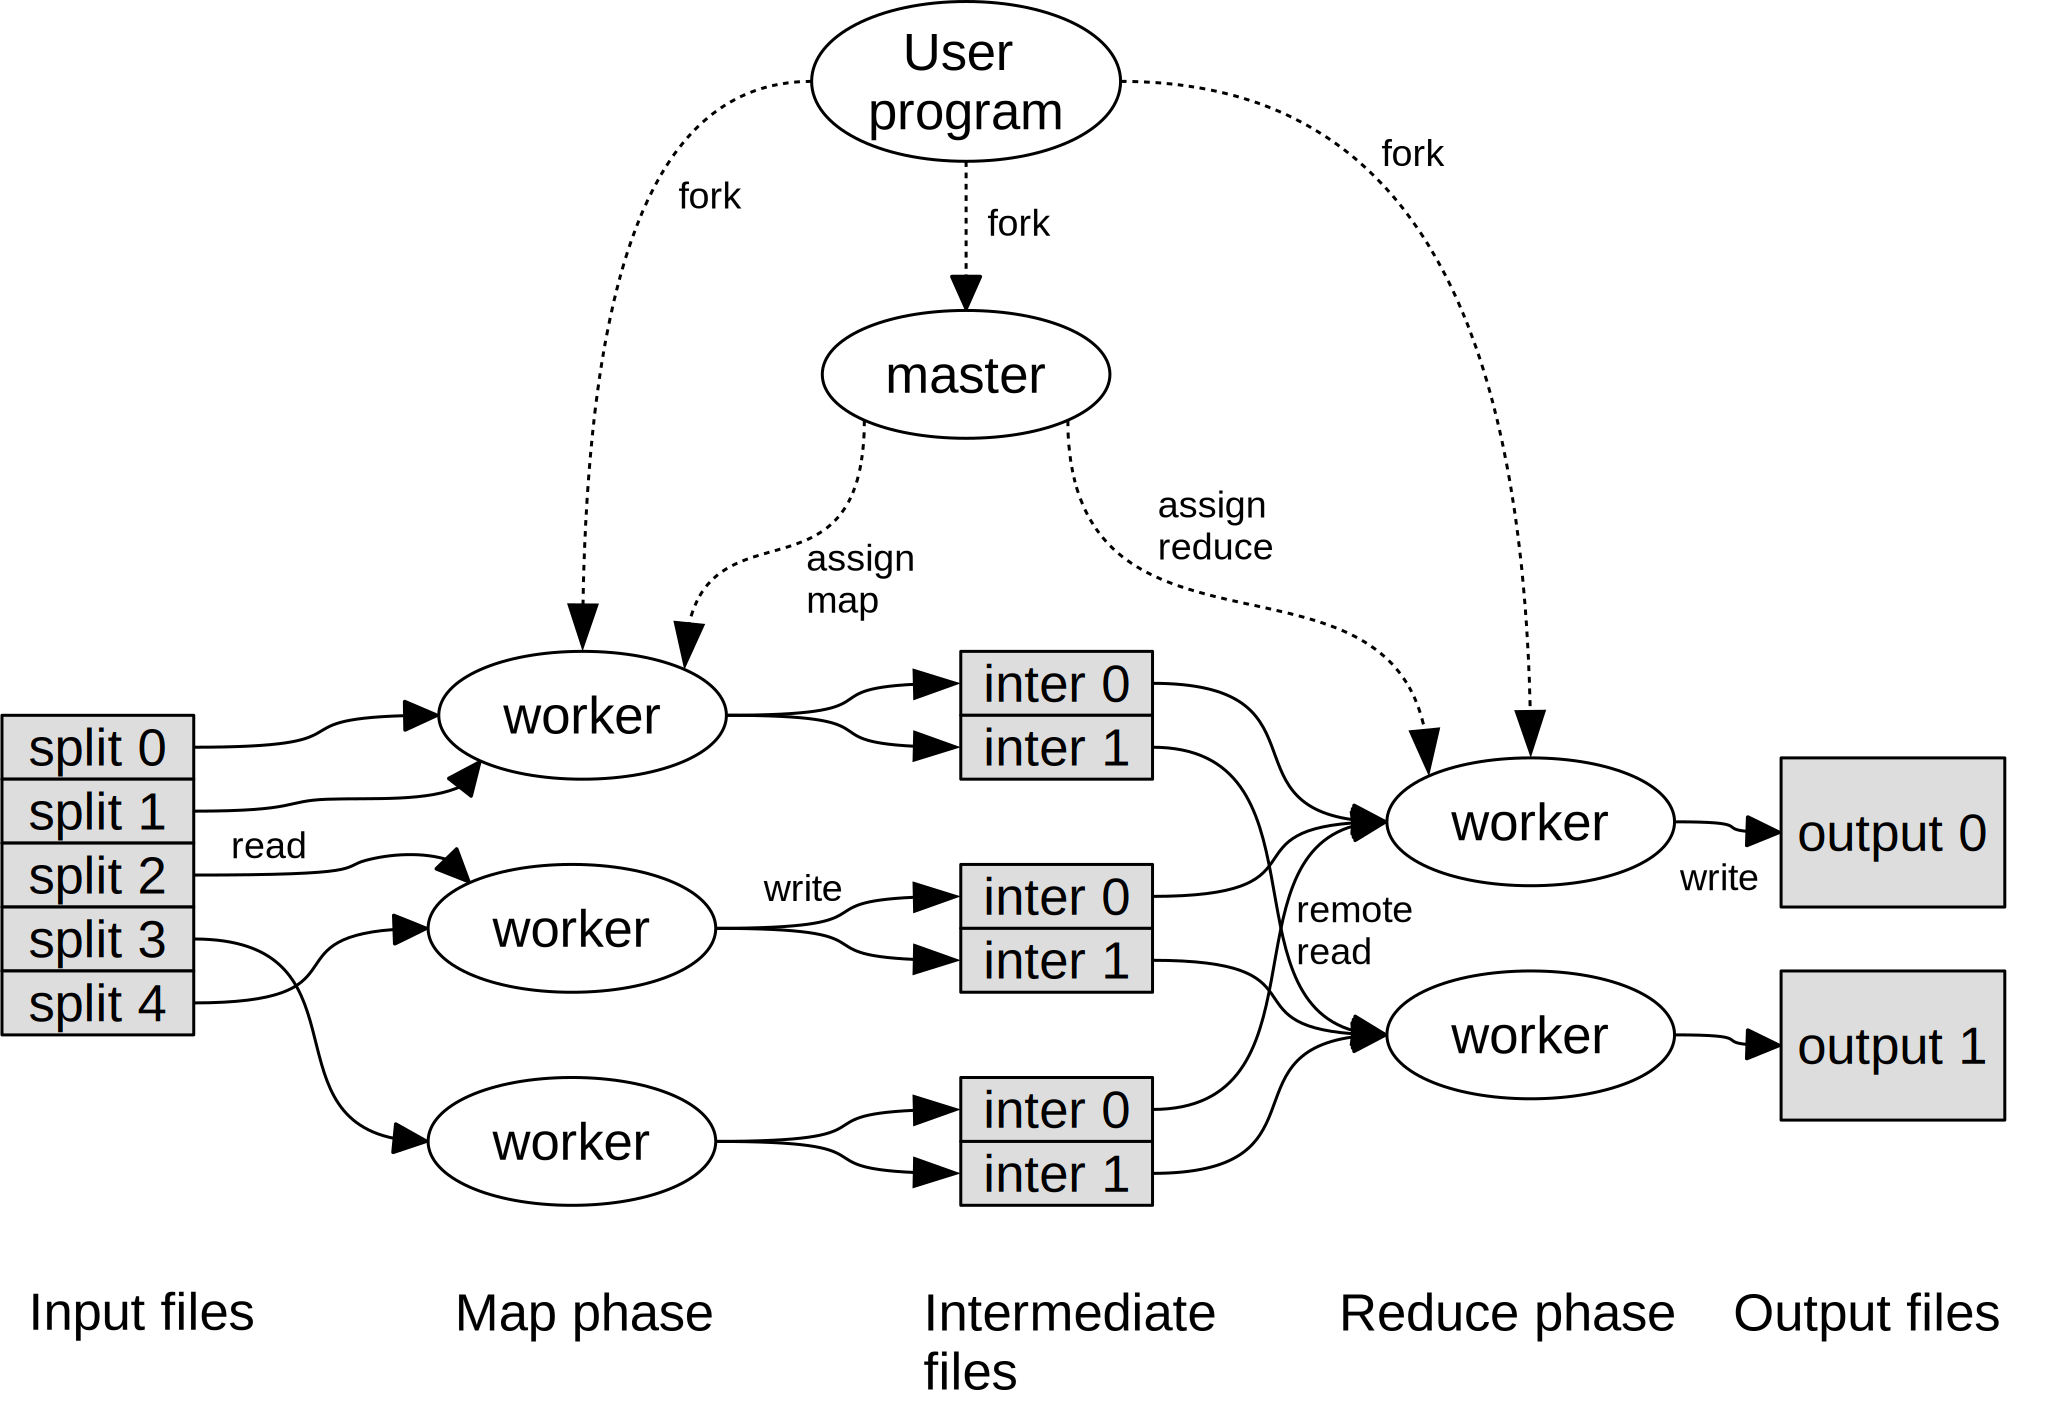
\includegraphics[width=1.0\textwidth]{images/mapreduce.pdf}
\caption{MapReduce-Laufzeitumgebung wie von Google vorgeschlagen. \cite{miner2012mapreduce}}
\label{fig:mapreduce}
\end{figure}

Die Verarbeitung von Daten mittels MapReduce läuft dann folgendermaßen ab:

Die Eingabedateien werden in $M$ gleich große Teilstücke von üblicherweise $16MB$ bis $64MB$
aufgeteilt. Das vom Nutzer implementierte \textit{User program} enthält die \textit{map}- und 
\textit{reduce}-Funktionen. Die einzelnen Maschinen (\textit{worker}) im Cluster bekommen jeweils
eine Kopie des Programms. Dabei ist eine einzige Kopie der Master, der sich anschließend
um die Koordination der Arbeit kümmert. Mit den $M$ gleich großen Teilstücken stehen nun
auch $M $ map-Aufgaben bereit zur Verarbeitung. Anschließend wird auch die Anzahl der Teilstücke
der Zwischenergebnisse $R$ ermittelt. Diese Anzahl $R$ stellt dann die Menge der verfügbaren
\textit{reduce}-Aufgaben dar.

Nach dieser Vorbereitung kann die Arbeit nun schließlich beginnen. Dafür schaut der Master nach,
welche Maschinen beziehungsweise Worker nicht beschäftigt sind und weist ihnen entweder eine \textit{map}- oder \textit{reduce}-Aufgabe zu. Die Map-Worker beginnen nun
die ihnen zugewiesenen Dateien zu bearbeiten, die aus Schlüssel-Wert-Paaren bestehen und
erzeugen die Zwischen-Dateien. Die Zwischen-Ergebnisse sind ebenfalls nach Schlüssel-Wert-Paaren
strukturiert. Die Zwischen-Ergebnisse werde dabei in $R$ Teil-Bereiche eingeordnet, abhängig
von ihrem Schlüssel-Wert.

Sobald ein oder mehrere map-Aufgaben erledigt sind, teilt der Master ein oder mehreren 
reduce-Workern, die gerade nichts zu tun haben, mit, dass sie mit der Verarbeitung beginnen können. Der Master teilt ihnen dabei auch mit, wo die entsprechenden Zwischenergebnisse liegen,
die sie verarbeiten sollen. Die reduce-Workers verarbeiten nun diese Dateien und erzeugen
mit ihrer Ausgabe einen Teil des End-Ergebnisses.


\subsection{Beispiel}
Als Beispiel dient die Analyse einer großen Datenmenge von Musiksongs mit Hilfe von MapReduce. Die Daten liegen als
Schlüssel-Wert-Paare vor. Jeder Song hat dabei einen eigenen Schlüssel, die Song-ID, sowie eine Reihe von Song-Informationen als Wert.
Die Song-Informationen beinhalten Daten wie Name des Songs, der Künstler, Beats-per-Minutes, aktueller Rank in den Charts etc.

Wir wollen nun in diesem sehr großen Datensatz an Songs herausfinden, welcher Künstler wie viele Songs geschrieben hat. Wir gehen in diesem Beispiel davon aus, dass wir eine Kenntnis davon haben, welche Künstler in  dem Datensatz vorkommen.
Im ersten Schritt müssen wir die \textit{map}-Funktion beschreiben. Sie bekommt als Eingabe eine Reihe von Songs mit der Song-ID
als Schlüssel und ihren Eigenschaften als Werte. Diese Songs werden nun direkt auf ein Zwischenergebnis gemappt, indem der
Künstler-Name als Schlüssel und die Zahl $1$ als Wert geschrieben werden. Dies führt zu einem (großen) Zwischenergebnis,
bei dem die Anzahl der Vorkommnisse eines Künstler-Names die Anzahl seiner Songs wiedergibt. Das muss aber
natürlich noch als End-Ergebnis zusammen gefasst werden, was dann die \textit{reduce}-Funktion übernimmt. 

Die \textit{reduce}-Funktion bekommt vom Master einen Werte-Bereich aus dem Zwischen-Ergebnis zugewiesen, die sie auf
ein End-Ergbnis reduzieren soll. Sie holt sich dann anschließend diesen Wertebereich des Zwischen-Ergebnisses von den verteilten
\textit{map}-Maschinen. Sie fasst nun alle gleichen Schlüssel zu einem einzigen Schlüssel zusammen und addiert 
ihren Wert jeweils auf. Da der Wert immer $1$ ist, steht am Schluss neben dem Künstler-Name die Anzahl seiner geschriebenen
Songs. Dieses Ergebnis schreibt die  \textit{reduce}-Funktion nun als Ergebnis raus. Die Abbildung \ref{fig:mapreduceExample} zeigt 
das Beispiel anschaulich.

\begin{figure}
\centering
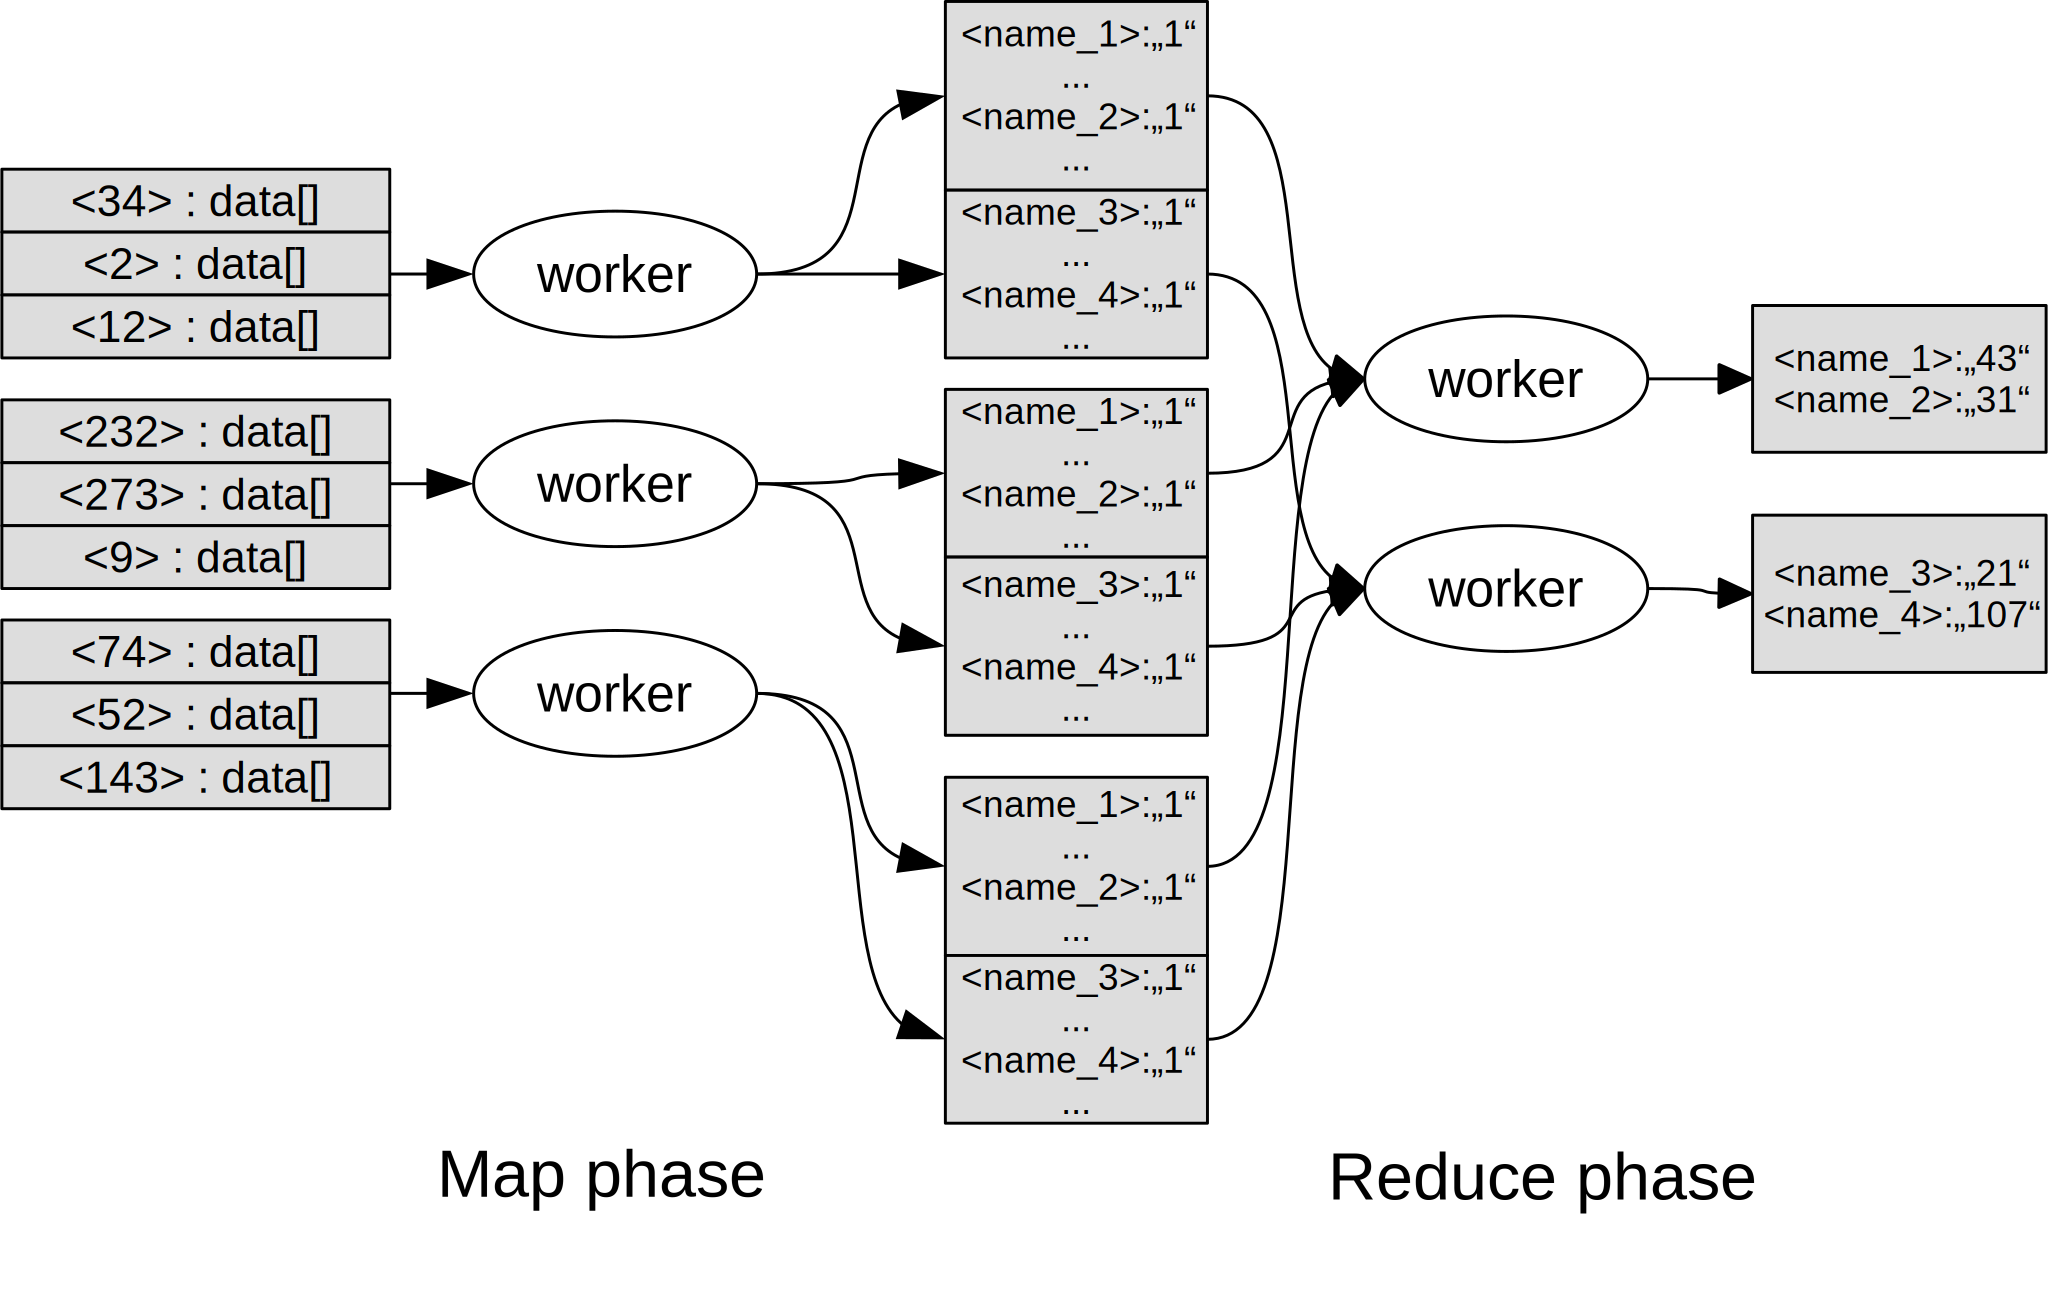
\includegraphics[width=1.0\textwidth]{images/mapreduceExample.pdf}
\caption{Ermittlung der Anzahl der Songs für jeden Künstler mittels MapReduce.}
\label{fig:mapreduceExample}
\end{figure}

%\subsection{Implementierung von MapReduce-Funktionen}

Dieser Abschnitt beschreibt die Implementierung von Map-Reduce-Funktionen, die auf den Daten
des Million-Song-Datensatzes arbeiten. Vorausgesetzt wird, dass der Million-Song-Datensatz als
CSV-Datei bereit in das HDFS-Dateisystem importiert ist. Die hier vorgestellten MapReduce-Funktionen
arbeiten ausschließlich mit Daten auf dem HDFS-Dateisystem, abgesehen von den Zwischenergebnissen,
die auf dem lokalen Dateisystem des jeweiligen Knotens abgelegt werden.
Für die Implementierung wird die Java-API des MapReduce von Hadoop verwendet. Wichtig ist,
dass die aktuelle MapReduce-API verwendet wird, und nicht die inzwischen veraltete MapRed-API.
Eine gute Hilfe bei der Entwicklung von map- und reduce-Funktionen bietet \cite{miner2012mapreduce}.

Die erste Implementierung der MapReduce-Funktionen überführt alle Songs aus der ursprünglichen
CSV-Datei in eine neue CSV-Datei, in der erstens kein Song mehr doppelt vorkommt und zweitens
ein Song nur noch eine Untermenge der ursprünglichen Attribute enthält. Damit soll der ursprüngliche
Datenbestand auf einen reduzierten Datenbestand mit den für den Nutzer interessanten Attributen 
transformiert werden. Die map-Funktion ist dafür verantwortlich, die Attribute eines Musikstückes
zu identifizieren und daraus mit einen neuen Musikstück-Eintrag zu erzeugen, der nur noch die interessanten
Attribute enthält.
Zuerst muss definiert werden, welche Eingabeparameter die map-Funktion bekommt. Dazu gibt es verschiedene
Eingabeformate der MapReduce-API, unter denen man wählen kann. Weil die Daten in der CSV-Datei für das
MapReduce-Framework nichts weiter als reiner Text ist, wird das \textit{Text}-Format als Eingabe für
die map-Funktion gewählt, welches gleichzeitig auch das Standard-Format für die map-Funktion ist.
Das Format des Schlüssel-Parameters wird nicht weiter angegeben, weil der Schlüsselwert in diesem Falle 
während der Verarbeitung keine Rolle spielt.
Die map-Funktion teilt den übergebenen Wert des Textes in die Song-Attribute auf, indem es den Text
als einzelnen String betratet und mittels der \textit{split}-Methode ein Feld von String erzeugt, die durch
das Komma im String getrennt sind. Dadurch sind die Musik-Attribute als Strings nun einzelnen verfügbar.
Der neue Eintrag für den Song wird durch das Erzeugen eines neuen Strings und dem Anhängen ausgewählter
Attribute erzeugt. Ist der neue String fertig zusammen gebaut, wird er wieder in das hadoop-spezifische \textit{Text}
konvertiert und als Zwischenergebnis dem MapReduce-Framework übergeben. Dieses erwartet neben dem 
Wert aber auch einen Schlüssel. Der Schlüssel ist in dem Falle ebenfalls vom Typ \textit{Text}, der als Wert die
Song-ID des Musikstückes enthält.

\lstset{
    language=Java,
    basicstyle=\ttfamily,
    frame=single,
    breaklines=true,
    postbreak=\raisebox{0ex}[0ex][0ex]{\ensuremath{\hookrightarrow\space}}
}

\begin{lstlisting}
  protected void map(Object key, Text value, Context context) {
      String[] allAttributes = value.toString().split(",", maxNumOfAttr);
      String newStrippedValue = new String();
      songId.set(allAttributes[songIdColumn-1]);
      
      for(int i=0; i<untilGenreAttr; i++){
          newStrippedValue += ","+allAttributes[i];
      }
      
      for(int k=fromGenreAttr-1; k<maxNumOfAttr; k++){
          newStrippedValue += ","+allAttributes[k];
      }
      
      strippedSongAttr.set(newStrippedValue);
      context.write(songId, strippedSongAttr);
   }
\end{lstlisting}



%Kein Thema in diesem Kapitel zugeordnet
\chapter{Ausgewählte Persistenzmodelle}
%\input{2.06.00}
\chapter[Ausgewählte Persistenzsysteme]{Ausgewählte Persistenzsysteme und Big Data Frameworks}
%Hadoop-Kapitel
\section{Hadoop}
%\cite{Wartal2012}
%\cite{Endlich2011}
\subsection{Visitenkarte}%alles ohne Technologie
Hadoop ist ein Java basiertes Open Source Framework von Apache. 
Die Entwicklung von Hadoop wurde als Teilpojekt von Nutch angefangen. Nutch selber ist eine Weiterentwicklung von Apache Lucene. Das Ziel des Projektes Nutch war es eine schnelle Websuche, also eine Alternative zu Google, zu entwickeln. Die Herausforderung für die Nutch Entwickler war hierbei die Erstellung eines Systems, welches mit hoch skalierbaren Prozessen, Redundanzen, automatischer Fehlerbeseitigung und Lastverteilung umgehen kann. Als Google im Jahr 2004 MapReduce und das \ac{GFS} Konzept vorgestellt hat, erkannte Doug Cutting, der Erfinder von Nutch, die Vorteile und hat sie für Nutch übernommen. Im Jahr 2006 wurde Doug Cutting von Yahoo, seinem damaligen Arbeitgeber, damit beauftragt das verteilte Dateisystem und das MapReduce-Framework aus dem Nutch-Kontext zu extrahieren und in ein eigenes Framework zu überführen. So entstand Hadoop, dessen Name von dem Spielelefanten von Doug Cuttings Sohn stammt. Im Juli 2008 gewann Hadoop den Terabyte-Sort-Benchmark, was bereits damals die Reife des entstandenen Projektes zeigte. \cite[S. 24]{Wartal2012}

Mit den neuen Konzepten von Google ermöglicht Hadoop das Verteilen der Verarbeitung komplexer Prozesse über mehrere Knoten innerhalb eines Clusters.
Die Hauptziele von Hadoop sind:

\begin{itemize}
\item Erreichbarkeit: Hadoop läuft in einem großen Cluster von Rechnern oder in einer Cloud 
\item Robustheit: Wenn ein Knoten ausfällt, übernehmen andere Knoten die Verarbeitung der Daten
\item Skalierbarkeit: Hadoop skaliert linear. Es können dynamosch weitere Rechner dazugeschaltet werden, um damit die Performance des Systems zu verbessern.
\item Einfachheit: Hadoop ermöglicht eine schnelle Entwicklung der parallelen Prozesse.
\cite{HadoopInAction}
\end{itemize}

%------------------------------------------------------------------------------------------------------------------------------------------------------------------------------------------------------------------------------------------------

\subsection{Systemtechnologie}
Hadoop besteht aus mehreren Modulen, die im Weiteren kurz beschrieben werden:

\begin{figure}[htbp] 
  \centering
     \includegraphics[width=0.5\textwidth]{images/06hadoop_modules.png}
  \caption{Hadoop-Module \cite{HaMo}}
  \label{fig: Hadoop-Module}
\end{figure}

\begin{itemize}
\item Hadoop Common: Hadoop Common stellt die Grundfunktionen bereit, die alle anderen Komponenten benötigen. Dazu zählen eine implementierungsneutrale Filesystem-Schnittstelle, die Schnittstelle für die "Remote Procedure Call"-Kommunikation im Cluster und Bibliotheken für die Serialisierung von Daten.
\item Hadoop YARN: Ein Modul für das Job-Scheduling und Cluster-Resource-Maagement
\item \ac{HDFS}: Verteiltes Dateisystem, welches einen hoch perfomanten Zugriff auf die Daten bereitstellt.
\item Hadoop MapReduce: Es ist ein auf YARN- basiertes System für die parallele Verarbeitung von riesigen Datenmenge.
\end{itemize}
Es ist möglich, Hadoop mit mehreren Dateisystemen zu betreiben: FS, HFTP FS, S3 FS etc. Das gängigste Dateisystem ist aber das \ac{HDFS}. Dieses Dateisystem basiert auf dem Google File System (\ac{GFS}). 
HDFS verwendet eine Master / Slave Architektur. Dabei verwaltet der Masterknoten (NameNode) die Metadaten von dem Dateisystem. Die Slave Knoten (DataNode) speichert die aktuellen Daten.
\subsubsection{NameNode}
Der \textit{NameNode} verwaltet alle Dateioperationen im Hadoop-Cluster. Er beinhaltet Information über die Unterteilung der Daten in Blocks und auf welcehn Knoten die Blöcke gespeichert werden.
Die Prozesse des  \textit{NameNodes} sind sehr Speicher- und I/O-lastig. Deswegen sollten \textit{NameNodes} keine Benutzerdaten speichern oder in den Berechnungsprozess eingebunden sein. Daraus resultiert, dass ein Rechner nicht gleichzeitig NameNode und DataNode sein sollte.
Zusammengefasst sind die Hauptaufgaben des NameNodes im Hadoop Dateisystem  \cite[S. XX]{Wartal2012}:
\begin{itemize}
\item Speicherung von Metadaten des Dateisystems im Hauptspeicher
\item Koordinierte Verteilung der einzelnen Datenblöcke
\item Überwachung der einzelnen Rechner-Knoten , um einen Ausfall schnell erkennen zu können
\end{itemize}

Alle Daten werden in Blöcke je 64 MB aufgeteilt. Im Vergleich zu gängigen Dateisystemen ist dies eine sehr großzügige Aufteilung. Zum Beispiel unterteilt das Linux Dateisystem alle Daten in 1KB große Blöcke. Die Aufteilung in solche großen Blöcke bei Hadoop basiert auf der Notwendigkeit sehr große Mengen an Informationen zu verarbeiten. Um einen Datenblock zu verarbeiten benötigt ein \textit{NameNode} in der Regel 150Byte Arbeitsspeicher. Demnach kann ein 1GB großer Arbeitsspeicher mehr als 6 Mio Dateien und Ordner verwalten. \cite[S. XX]{Wartal2012}
\subsubsection{DataNode}
Ein \textit{DataNode}, auch Slve-Knoten genannt, ist für die Speicherung der Daten in \ac{HDFS} verantwortlich. Er berichtet dem \textit{NameNode} über den Status der Datenverarbeitung in regelmäßigen Abständen und meldet sich bei seinem Start bei ihm an. Die Daten werden auf mehrere \textit{DataNodes} repliziert, um die Ausfallsicherheit gewährleisten zu können.
Ein\textit{DataNode} benötigt sehr viel Speicherkapazität, weil alle Daten ihm gespeichert sind \cite{nameNode}.


\subsubsection{SecondaryNameNode}
Um die Aufgabe eines \textit{SecondaryNameNodes} zu verstehen, betrachten wir kurz welche Dateien von einem \textit{NameNode} geschrieben werden und welche Probleme dabei entstehen:
\begin{figure}[H]
	\centering
	\includegraphics[width=1.0\textwidth]{images/{06.namenode}.png}
	\caption{Funktionsweise eines \textit{NameNodes}}
	\label{img:grafik-nameNode}
\end{figure}

Wie aus der Abbildung zu sehen ist, schreibt ein \textit{NameNode} zwei unterschiedliche Dateien auf die Festplatte: \\
\begin{itemize}
\item Das \textit{FsImage} ist eine Moment-Aufnahme des Dateisystem zum Zeitpunkt des Starts der \textit{NameNodes}
\item Der \textit{EditLog} beinhaltet die Änderungen, die nach dem Starten eines \textit{NameNodes} auftreten.
\end{itemize}
Ein FsImage wird nur beim Neustart eines \textit{NameNodes} erzeugt. Dabei wird die Information aus dem \textit{EditLog} in einen FsLog (FileSystem-Log) geschrieben, um die Moment-Aufnahme des Dateisystems zu speichern. Dadurch wird die Zeit für den Neustart des Systems beschleunigt.
Da in der Regel ein \textit{NameNode} nur sehr selten neu gestartet wird, entstehen folgende Probleme:
\begin{itemize}
\item Der \textit{EditLog} wird sehr groß und kann nicht verwaltet werden.
\item Das Neustarten eines \textit{NameNodes} dauert aufgrund der großen Datenmenge sehr lange.
\item Im Falle eines Ausfalls des \textit{NameNodes} geht eine sehr viele Daten verloren.
\end{itemize}

Der \textit{SecondaryNameNode} wird benötigt, um diese Probleme zu umgehen.\\
\begin{figure}[htbp]
	\centering
	\includegraphics[width=1.0\textwidth]{images/{06.secondarynamenode}.png}
	\caption{Funktionsweise eines \textit{SecondaryNameNodes}}
	\label{img:grafik-SecondaryNameNode}
\end{figure}

Die Aufgaben eines \textit{SecondaryNameNodes} sind also  \cite{secNameNode}:
\begin{itemize}
\item Daten in regelmäßigen Abständen vom \textit{EditLog} ins \textit{FsImage} verschieben.
\item Sobald ein neues \textit{FsImage}  vorhanden ist, wird es auf den \textit{NameNode} geschrieben.
\item Das neue \textit{FsImage}  wird beim nächsten Neustart des \textit{NameNodes} verwendet.
\end{itemize}

\subsubsection{Replikation der Daten in Hadoop}
Hadoop verwendet einen blockorientierten Ansatz für die Datenreplikation. Mit disem Ansatz wird jede im \ac{HDFS} abgelegte Datei in einzelne Blöcke mit einer festen Bytegröße aufgeteilt und durch den \textit{NameNode} auf unterschiedliche Cluster-Knoten abgelegt. Zusätzlich wird durch den \textit{NameNode} sichergestellt, dass jeder Block mehrfach auf unterschiedliche Knoten im Cluster repliziert wird.
In der HDFS-Standardkonfiguration repliziert der \cite{replikation} jeden Block dreifach. Kommt es nun zum Ausfall eines Knotens im Cluster, gehen nur die auf dem ausgefallenen Rechner vorhandenen Blöcke verloren und keine ganze Datei. Die verloren gegangenen Blöcke werden durch ihre Kopien auf anderen Knoten ersetzt, sodass der \textit{NameNode} die ganze Datei bereitstellen kann \cite{replikation}.


%------------------------------------------------------------------------------------------------------------------------------------------------------------------------------------------------------------------------------------------------

\subsection{Datenmodell}
In diesem Projekt wird im Bezug auf die Datenmodellierung lediglich das \ac{HDFS} aus dem Hadoop-Framework für das Speichern der Dateien genutzt. 

%------------------------------------------------------------------------------------------------------------------------------------------------------------------------------------------------------------------------------------------------

\subsection{Systeminstallation} % Installation auf der Grundlage unseres Clusters
Da Hadoop in Java implementiert ist, ist es plattformunabhängig und kann sowohl auf Windows, Linux oder MacOs installiert werden.
Im folgenden Abscnitt wird beschrieben, wie man Hadoop auf mehreren Knoten innerhalb eines Clusters installieren kann. 

Bevor man mit der Installation von Hadoop System begint, müssen zwei Voraussetzungen erfüllt werden.
\begin{enumerate}
\item Eine Java Laufzeitumgebung. Für Hadoop braucht man mindestens Java Version 1.6.
Nachdem Java auf der dafür vorgesehenen Maschine installiert ist, muss man die \textit{JAVA\_HOME}-Variable mit dem richtigen Java-Verzeichnis verknüpfen.
\item \ac{SSH} muss installiert werden und der \textit{\ac{SSH}-Daemon} muss laufen, damit die Hadoop-Scripte ausgeführt werden können.
\end{enumerate}
Als nächstes muss eine Hadoop-Distribution aus dem Internet (\url{http://hadoop.apache.org/releases.html}) geladen und für den \textit{Single}- oder \textit{MultipleMode} konfiguriert werden. Bei einer Cluster-Installation muss Hadoop auf jeden Knoten des Clusters installiert werden.
Die Konfiguration von Hadoop wird an zwei Stellen verteilt \cite{hadoopConfiguration}:
\begin{itemize}
\item Read-only default configuration - core-default.xml, hdfs-default.xml, \\yarn-default.xml and mapred-default.xml.
\item Site-specific configuration - etc/hadoop/core-site.xml,\\ etc/hadoop/hdfs-site.xml, etc/hadoop/yarn-site.xml and etc/hadoop/mapred-site.xml.
\end{itemize}


Sämtliche Konfigurationsdateien befinden sich in der Hadoop Version 2.7.3 im folgenden Verzeichnis: \textit{etc/hadoop/}:
\begin{itemize}
\item In der Datei \textit{hadoop-env} findet man einen Hinweis auf die installierte Java-Version, spezifischen Speichereinstellugen usw. 
\item Die Datei \textit{core-site.xml} beinhaltet das Verzeichnis und die Adresse des Hadoop-Dateisystems. Bei einer neuen Hadoop-Installation ist diese Datei leer und muss mit Inhalt befüllt werden.
\item Der Parameter \textit{hadoop.tmp.dir} legt fest, in welchem Verzeichnis Hadoop die benötigten Dateien für das HDFS anlegen darf.
\item Der Parameter \textit{fs.defaultFS} beschreibt den \ac{URI} des \textit{NameNodes}.
\item Die Datei \textit{hdfs-site.xml} bestimmt unter Anderem den Grad der Replikation innerhalb des \ac{HDFS}. Darüber hinaus kann man in dieser Datei den Pfad zum Verzeichnis finden, in dem die Daten vom \textit{NameNode} (\textit{dfs.namenode.name.dir}) und die Daten vom \textit{DataNode}(\textit{dfs.datanode.data.dir}) liegen.
\end{itemize}

Die vollständige Liste aller Konfigurationsparameter inklusive ihrer Default-Werte finden sich unter:

\begin{itemize}
	\item \url{https://hadoop.apache.org/docs/r2.7.2/hadoop-project-dist/
	hadoop-common/core-default.xml}
	\item \url{http://hadoop.apache.org/docs/r2.7.2/hadoop-project-dist/
	hadoop-hdfs/hdfs-default.xml}
	\item \url{https://hadoop.apache.org/docs/r2.7.2/hadoop-yarn/
	hadoop-yarn-common/yarn-default.xml}
\end{itemize}

%------------------------------------------------------------------------------------------------------------------------------------------------------------------------------------------------------------------------------------------------

\subsection{Datenschema}
Das logische Datenschema wird in Abschnitt \ref{hbase_datenschema}  beschrieben.

%------------------------------------------------------------------------------------------------------------------------------------------------------------------------------------------------------------------------------------------------

\subsection{Ad-Hoc-Zugriffsmöglichkeiten}
CRUD-Operationen können in Hadoop auch ohne HBase über einen Hive-Client durchgeführt werden. Dies war jedoch nicht Bestandteil dieses Projekts. CRUD-Operationen mit HBase werden in Abschnitt \ref{hbase_adhoc} beschrieben.

\newpage
%HBase-Kapitel
\section{HBase}

Im Folgenden wird HBase als \textbf{die} Hadoop Datenbank vorgestellt, die zu Grunde liegende Systemtechnologie erläutert  und die Installation/Konfiguration beschrieben.
\subsection{Visitenkarte}
\subsubsection{Entstehung}
Nachdem Google immer größer werdende Datenmassen speichern musste und dieses Problem mit dem  \ac{GFS} gelöst zu sein schien, stellten sich weitere Probleme heraus: 
Die Indexierung dieser Daten und die Verteilung der Daten auf viele Knoten ohne Zugriffgeschwindigkeit und Konsistenz zu verlieren. Google fand eine Lösung mit BigTable und auf Grundlage des veröffentlichten Whitepapers \cite{bigtable} dazu, entwickelte die Open-Source-Community HBase. Aus diesem Grund weisen diese beiden Datenbanken auch Gemeinsamkeiten bezüglich ihrer Funktionalität auf. Beispielsweise unterstützen beide die Komprimierung (siehe \ref{tableoperation}) und Versionierung der Daten \cite{SpaOd16}.

\subsubsection{Allgemein}
HBase wurde entwickelt, um mit Hadoop zusammen zu arbeiten, ist ein verteiltes BigData-Speichersystem 
 und bietet einen schnellen (nahe Echtzeit) Zugriff auf riesige Datenmengen.


\subsubsection{Portfolio}
HBase wird von vielen bekannten Konzernen eingesetzt, da es sich gut für Logging- und Suchsysteme eignet und als Grundpfeiler für \ac{OLAP}-Systeme geeignet ist \cite{Redt01}.

\begin{figure}[H] 
  \centering
     \includegraphics[width=0.7\textwidth]{images/{06.portfolio}.png}
  \caption{HBase-Portfolio \cite{youportf}}
  \label{fig:Portfolio}
\end{figure}

%------------------------------------------------------------------------------------------------------------------------------------------------------------------------------------------------------------------------------------------------

\subsection{Systemtechnologie} % ausgewählte technologische Aspekte (Architektur, Funktionsweise, ...) ohne (ausführliche) Modellierungsaspekte
 In HBase lassen sich riesige Datenmengen auf mehreren Knoten verteilen, verwalten und jederzeit erweitern. HBase basiert auf Java, ist Open-Source, nicht-relational, spaltenorientiert und setzt auf ein verteiltes Dateisystem wie \ac{HDFS} von Hadoop auf \cite{hbasetut}. HBase, als Key-Value-Store, wurde als fehlertolerantes System entworfen, das auch gut mit unvollständige Datenmengen umgehen kann. Aufgrund des schemalosen Datenmodells, müssen nicht alle Felder belegt werden und verbrauchen auch keinen Speicherplatz \cite{compWo}.  Durch das \ac{WAL} und eine verteilte Konfiguration kann sich HBase schnell von Serverausfällen erholen \cite{Redt01}. 
 
 Nach CAP-Theorem legt es besonders Wert auf Verfügbarkeit und Partitionierung und vernachlässigt die Konsistenz der Daten. 
 Des Weiteren unterstützt HBase die Replikation von Hadoop, den MapReduce-Algorithmus, automatische Verteilung der Tabellen auf die Knoten, Komprimierung der Daten und Bloom-Filter. HBase kann im Standalone-Modus, im pseudo-verteilten Modus und im vollständig-verteilten Modus betrieben werden. Für den vorliegenden Use case wird am Ende des Kapitels die Konfiguration für den vollständig-verteilten Modus beschrieben. Für diesen Modus wird für die verteilte Konfiguration ein Zookeeper benötigt (siehe Abschnitt \ref{zook}). HBase stellt zwar selbst keine SQL-API zur Verfügung lässt sich aber durch Schnittstellen wie Apache Phoenix um eben solche erweitern.

\subsubsection{HBase im Vergleich zu einem \ac{RDBMS}}
HBase erinnert an eine relationale Datenbank, da die Daten in Tabellen gespeichert werden, die Zellen enthalten. Jedoch verhalten sich die Tabellen nicht wie Relationen und die Zeilen nicht wie Datensätze in relationalen Datenbanken. Auch sind die Spalten nicht durch ein Schema definiert.
HBase speichert die teils unvollständigen Daten in Spalten ab im Vergleich zu vollständigen Reiheneinträgen in einem \ac{RDBMS}. Dies ist notwendig da große Datenmengen den Anforderungen auf Vollständigkeit, wie sie ein \ac{RDBMS} erfordert, oftmals nicht gerecht werden.  
Während in einem \ac{RDBMS} viele schmale, normalisierte Tabellen vorliegen, ist HBase für Tabellen mit Millionen von nicht-normalisierten Spalten ausgelegt. Die Partitionierung wird bei HBase automatisch vorgenommen, währenddessen in einem RDBMS dies manuell erfolgen muss \cite{youintr}. Durch die Spaltenorientierung ist
HBase besonders gut für analytische Aufgaben geeignet, da es selektiv nur die benötigten Daten abfragt und nicht die komplette Zeile, wie es ein \ac{RDBMS} tut.


\subsubsection{HBase im Vergleich zu HDFS}
Da HBase selbst seine Daten nicht speichern kann, bedient es sich der \ac{HDFS}-Funktionen (siehe Abschnitt \ref{hadooptech}). Im Unterschied zu normalen Dateisystemen wie ext4 oder NTFS kümmert  sich \ac{HDFS} automatisch um die Replikation von Daten zwischen den Knoten,  
sodass eine hohe Skalierbarkeit und eine hohe Ausfallsicherheit entsteht. Da HDFS ein Filesystem ist, fehlt ihm die zufällige Lese-und Schreibfähigkeit. Eine mögliche Lösung dafür ist HBase. Es stellt innerhalb des Clusters in Echtzeit Lese- und Schreibzugriff zu den Daten her. Zur Speicherung großer Binärdaten ist die direkte Nutzung von HDFS besser geeignet \cite{compWo}. 
Es wird empfohlen HBase in einem verteilten System ab fünf Knoten einzusetzen \cite{SpaOd16}.

\begin{figure}[H] 
  \centering
     \includegraphics[width=0.7\textwidth]{images/{06.architecture}.png}
  \caption{HBase-Architektur \cite{clo11}}
  \label{fig:architecture}
\end{figure}


\subsubsection{MasterServer}
HBase besitzt zwei Rollen: den HBase \textit{MasterServer} und die \textit{RegionServer}. Der \textit{MasterServer} ist verantwortlich für die Zuweisung der Regionen (siehe Abschnitt \ref{region}) an die \textit{RegionServer}, die Verteilung der Last (Abschnitt \ref{tableoperation}), den Neustart der \textit{RegionServer}, die Teilung (Abschnitt \ref{tableoperation}) und die Überwachung der \textit{RegionServer}. Es ist möglich mehrere \textit{MasterServer} in einem Cluster zu betreiben, wobei aber nur einer aktiv sein kann. Da der \textit{MasterServer} nur verwaltende Funktionen inne hält, kann ein Cluster auch ohne ihn arbeiten, solange kein \textit{RegionServer} ausfällt. Spätestens dann muss ein \textit{MasterServer} eingreifen und die Regionen neu zuweisen. Die Verfügbarkeit des \textit{MasterServers} wird vom Zookeeper verwaltet \cite{Redt01}.

\subsubsection{RegionServer}
Der \textit{RegionServer} beinhaltet die HBase Regionen (siehe \ref{region}) und die HBase-Daten, welche lexikographisch nach dem Reihenschlüssel sortiert  werden. Die Aufrufe der JAVA-API gehen direkt an die \textit{RegionServer}, damit der \textit{MasterServer} nicht als Flaschenhals agiert. Der \textit{RegionServer} komprimiert und verteilt die Daten und berichtet dem  \textit{MasterServer}. Es wird empfohlen nur einen \textit{RegionServer} pro Maschine zu betreiben \cite{Redt01}. Für Lese-und Schreibzugriffe kommuniziert der \textit{RegionServer} mit anderen \textit{RegionServern}.

\begin{figure}[H] 
  \centering
     \includegraphics[width=0.9\textwidth]{images/{06.cluster}.png}
  \caption{Exemplarische Aufteilung der Tabelle in Regionen}
  \label{fig:cluster}
\end{figure}


%------------------------------------------------------------------------------------------------------------------------------------------------------------------------------------------------------------------------------------------------

\subsection{Datenmodell} %Modellierungsaspekte

\subsubsection{Tabellen}\label{tabelle}
HBase speichert die Daten, ähnlich wie eine relationale Datenbank in Tabellen. Jedoch bestehen diese aus Reihenschlüsseln und Spaltenfamilien (siehe \ref{sf}). Es gibt zwei Arten von Tabellen: Die Benutzer-Tabellen und die System-Tabellen.
Die Systemtabellen werden für das Verwalten von Meta-Daten von \acp{ACL}, Tabellen, Regionen (siehe \ref{region}) und Namensräumen verwendet. Die Benutzer-Tabellen werden im vorliegenden Projekt für die Verwaltung des Million-Song-Dataset verwendet. Folgend ein Beispiel einer solchen Tabelle:

\begin{figure}[htbp] 
  \centering
     \includegraphics[width=0.7\textwidth]{images/{06.logisch}.pdf}
  \caption{Logische Darstellung der Daten}
  \label{fig:Logische Darstellung der Daten}
\end{figure}


\subsubsection{Regionen}\label{region}
Eine Tabelle besteht aus Spalten und Reihen. Für die Skalierung  und den randomisierten Zugriff, teilt HBase die Tabelle horizontal in Regionen auf, d.h. jede Region besteht aus einer Reihe von aufeinander folgenden Schlüsseln. Jede Region wird genau einem \textit{RegionServer} zugeordnet, um Konsistenz zu wahren. Der HBase Load-Balancer sorgt dafür, dass die Regionen auf alle \textit{RegionServer} gleich verteilt werden. Jede Region wird durch einen Start-Schlüssel und einen End-Schlüssel begrenzt. Diese Informationen lassen sich in den System-Tabellen wiederfinden. Regionen können geteilt werden, wenn sie zu groß werden oder zusammengelegt werden, wenn die zu klein sind.

\subsubsection{Spaltenfamilien}\label{sf}
Die Empfehlung ist, dass Daten mit gleichen Zugriffs-Queries und demselben Format in einer Spaltenfamilie zusammengefasst werden sollten. Wenn wir beispielsweise zu allen Songs des One-Million-Song-Datasets die Coverbilder der Songs hinterlegt hätten, könnten die Bilder in einer Spaltenfamilie und die textuellen Informationen zu den Songs in einer anderen Spaltenfamilie hinterlegt werden. So könnte die Spaltenfamilie mit den textuellen Informationen komprimiert werden (siehe Abschnitt \ref{tableoperation}). Wenn bestimmte Daten nur gelesen werden und andere meistens geschrieben werden, sollte ebenfalls über eine separate Spaltenfamilie nachgedacht werden. Es gibt keine Grenze nach oben für die Spaltenfamilien innerhalb einer Tabelle, jedoch leidet die Performanz bei vielen Spaltenfamilien. Der \textit{MemStore} (siehe \ref{memstore} wird dadurch belastet und generiert viele kleine Dateien. Bei der Tabellenerzeugung  muss bis auf die Spaltenfamilien keine feste Vorgabe gemacht werden. Alles außer der Tabellenname wird als Byte-Array abgespeichert, d.h. man kann Zeichen, Zahlen, Buchstaben usw. abspeichern. Um auf einen Wert zugreifen zu können, muss der Reihenschlüssel, die Spaltenfamilie, der Spaltenname und  Zeitstempel (optional) angegeben werden \cite{SpaOd16}. In der folgenden Abbildung ist zu sehen, wie HBase seine Daten abspeichert:

\begin{figure}[H] 
  \centering
     \includegraphics[width=0.9\textwidth]{images/{06.physisch}.pdf}
  \caption{Physische Darstellung einer Tabelle}
  \label{fig:Physische Darstellung einer Tabelle}
\end{figure}

\subsubsection{Spalten}
Spalten werden nicht durch eine Schema-Beschreibung vorgegeben und können jederzeit zu einer Spaltenfamilie hinzugefügt werden. Jede Spalte kann mehrere Versionen (Abschnitt \ref{versionen}) erhalten. 

\subsubsection{Stores}
Es gibt einen Store pro Spaltenfamilie. Ein Store gruppiert den \textit{MemStore} und \textbf{0-n} \textit{Store}-Files (HFiles). 

\subsubsection{MemStore}\label{memstore}
Wenn Daten hinzugefügt oder geändert werden, wird ein \ac{WAL} erzeugt und in den \textit{MemStore} geschrieben, wo der Eintrag lexikographisch einsortiert wird. Ist der Im-Memory Speicher des \textit{MemStore} voll, werden die Daten als HFile im \ac{HDFS} abgespeichert. Die Logdateien im \textit{MemStore} werden erst gelöscht, wenn alle Änderungen festgeschrieben wurden. So wird sichergestellt, dass die Daten nicht verloren gehen, falls ein Knoten abstürzt.

\subsubsection{HFiles}
HFiles (Key-Value-Map) werden erzeugt, wenn die \textit{MemStores} voll sind und werden im HDFS abgespeichert, um von der Hadoop-Persistierung und Replikation zu profitieren. HFiles bestehen aus Blöcken. Ein Block hat eine Größe zwischen 8KB und 1 MB. Die Blockgröße kann konfiguriert werden.  Die Standard-Größe liegt bei 64KB. Es gibt viele Blocktypen die innerhalb eines HFiles vorkommen können: Der Datenblock enthält sowohl die Daten als auch die \textit{Put- und Delete-Markierungen}. Indexblocks ermöglichen das schnelle Auffinden einer Reihe innerhalb eines HFiles. Bloom-Filter-Blocks werden für das Überspringen von  bestimmten Parse-Vorgängen genutzt, damit der angefragte Schlüssel schneller gefunden werden kann. Trailer Blocks enthalten die HFile-Version. 
%HFiles sind unveränderlich, da HDFS kein Update erlaubt.
Zusammenfassende eine Darstellung der HBase-Architektur:

\begin{figure}[H] 
  \centering
     \includegraphics[width=1\textwidth]{images/{06.regionserverinternals}.png}
  \caption{RegionServer-Interna \cite{carmc}}
  \label{fig:Internals}
\end{figure}

\subsubsection{Interne Tabellenoperationen }\label{tableoperation}
Die große Stärke von HBase ist es, Daten zu größeren Dateien zusammenzufassen und Tabellen automatisch auf mehrere Rechner zu verteilen. Hierzu verwendet HBase drei verschiedene Mechanismen.
\begin{description}
\item[Komprimierung]
 Um zu vermeiden, dass beim \textit{Memstore-Flush} (siehe \ref{memstore}) viele kleine HFiles entstehen, legt HBase sie zu größeren Dateien zusammen.  Alle Dateien mit dem gleichen Schlüssel, aber einem älteren Zeitstempel werden so gelöscht. Beim Löschen von Zellen setzt HBase einen Marker, der bei der Komprimierung überprüft wird. In einer weiteren Stufe der Komprimierung können alle Marker gelöscht werden. Eine solche Komprimierung kann manuell für eine spezifische Region oder Tabelle angestoßen werden. Außerdem werden standardmäßig wöchentlich solche Komprimierungen von HBase selbst ausgeführt \cite{SpaOd16}.

\item[Teilung]
Das Gegenteil der Komprimierung ist die Teilung (Split), auch \textit{Auto-Sharding} genannt. Wenn eine Region eine Größe von 10GB erreicht, führt HBase eine Teilung durch und es entstehen zwei neue Regionen. Hierbei ist zu beachten, dass Teilungen immer spaltenfamilienübergreifend stattfinden \cite{SpaOd16}:

\begin{figure}[H] 
  \centering
     \includegraphics[width=0.7\textwidth]{images/{06.split}.pdf}
  \caption{Zwei Spaltenfamilien vor und nach der Teilung}
  \label{fig:Teilung}
\end{figure}


\item[Verteilung der Last]
Eine Verteilung der Last ist insbesondere bei der Neuordnung von Daten (Komprimierung) oder der Veränderung der Cluster-Umgebung (neuer oder gelöschter Rechnerknoten) notwendig.
HBase, um genau zu sein Hadoop, führt alle fünf Minuten einen LoadBalancer aus der algorithmisch sicherstellt, dass alle \textit{RegionServer} eine ähnliche Anzahl an Regionen bedienen \cite{SpaOd16}. 
\end{description}

 \subsubsection{Versionierung}\label{versionen}
Eine Reihe, eine Spalte und ein Zeitstempel spezifizieren exakt eine Zelle in HBase. Während Spalten und Reihen gleich bleiben können, ändert sich der Zeitstempel für jede Zelle. Der Zeitstempel, als Long-Integer-Datentyp, wird in absteigender Reihenfolge hinterlegt, sodass immer der aktuellste Wert aus den HFiles gelesen wird \cite{reference}.
Standardmäßig können drei Versionen einer Zelle erstellt werden.


\subsubsection{Zugriff auf HBase}
Obwohl aus Performanzgründen empfohlen wird die JAVA-API für den Zugriff auf HBase zu nutzen, werden im Folgenden weitere Möglichkeiten vorgestellt.
\begin{description}
\item[Thrift Server]
Der Thrift Server kann als Gateway benutzt werden, um Applikationen  anderer Sprachen, den Zugriff auf HBase zu ermöglichen. Ein C/C++ Client könnte bei dieser Lösung jedoch nur mit dem Thrift Server kommunizieren und nicht direkt auf einen \textit{RegionServer} zugreifen.

\item[REST Server]
HBase stellt auch eine REST-API zur Verfügung, auf die über HTTP zugegriffen werden kann.

\item[Hive] Mit Hilfe von SQL-Queries ist ein Zugriff auf HBase möglich, jedoch auf Kosten der Performanz (4-5mal langsamer) \cite{clo11}.
\end{description}

%------------------------------------------------------------------------------------------------------------------------------------------------------------------------------------------------------------------------------------------------

\subsection{Systeminstallation} %Installation auf der Grundlage unseres Clusters 
Für die Installation werden sowohl auf dem  \textit{MasterServer} als auch auf den \textit{RegionServern} folgende UNIX-Kommandos abgesetzt:
\noindent 
\begin{lstlisting}[language=bash]
  $ wget http://www-us.apache.org/dist/hbase/stable/
    hbase-1.2.4-bin.tar.gz
  $ tar -xzf hbase-1.2.4-bin.tar.gz
  $ ln -s hbase-1.2.4 hbase
  $ cd hbase
  $ export PATH=$PATH:~/hbase/bin
\end{lstlisting}

Die Konfiguration für HBase wird in einer Datei namens \textit{hbase-site.xml} erstellt. Hier werden Zookeeper-Einstellungen vorgenommen, das HDFS-System referenziert und der Betriebsmodus sowie der Pfad zur Datenspeicherung eingestellt.
Um HBase zu starten, wird der Befehl 
\noindent 
\begin{lstlisting}[language=bash]
  $ {HBASE_HOME}/bin/start-hbase.sh 
\end{lstlisting}
ausgeführt. HBase lässt sich mit dem Standard-Port 16010 durch folgenden \ac{URL} über die Weboberfläche aufrufen: \textit{localhost:16010}

\subsubsection{ZooKeeper}\label{zook}
ZooKeeper ist ein Open-Source-Projekt unter der Apache-Foundation. Typische Aufgabenstellungen sind:
\begin{itemize}
\item Wettlaufsituationen beim verteilten Schreiben auf denselben Daten zu lösen
\item Den Zugriff auf schon veraltete Daten zu regeln 
\item Das Auffinden von Rechnerknoten (\textit{RegionServern}) in einem Cluster
\item Überwachung der einzelnen Knoten im Cluster durch sogenannte \textit{Heartbeats}. Dies sind kurze Signale an den  \textit{MasterServer}, die signalisieren, dass der Rechnerknoten noch aktiv ist. 
\end{itemize}

Die Installation von ZooKeeper ist verhältnismäßig einfach. Nachdem die Anwendung auf die einzelnen Knoten herunter geladen ist, muss in der Datei \url{zookeeper/conf/zoo.cfg}
die Konfiguration erfolgen, die im einfachsten Falle nur aus der Angabe der Rechner-Knoten besteht. Innerhalb von ZooKeeper nennt sich so ein Verbund
von Rechner-Knoten ein \textit{esemble}. Diese Konfiguration muss anschließend auf alle Knoten verteilt werden. Danach kann der ZooKeeper-Server, genannt \texttt{zkServer},
auf jedem Knoten manuell gestartet werden. 

Über den Client-Port von ZooKeeper, der in diesem Projekt auf jedem Knoten der Port $2186$ ist, können die verteilten
Anwendungen die ZooKeeper-API verwenden. Dabei können sie sogenannte \textit{zNodes} anlegen. Das sind Dateien, auf die verteilt zugegriffen wird und um dessen
Gültigkeit sich nun ZooKeeper kümmert, sodass die verteilte Anwendung sich nicht mehr um die typischen Probleme, die in einem Cluster auftauchen, kümmern muss.

%------------------------------------------------------------------------------------------------------------------------------------------------------------------------------------------------------------------------------------------------

\subsection{Datenschema}\label{hbase_datenschema}
Für das Semesterprojekt wurde eine Tabelle mit dem Namen \textbf{music} angelegt. Diese enthält zwei Spaltenfamilien. Die Spaltenfamilie \textbf{song} enthält die für die Use cases (siehe Abschnitt \ref{usecases}) benötigten Daten und die Spaltenfamilie
\textbf{miscellaneous} enthält die restlichen Daten des Million-Song-Datasets:

\begin{figure}[H] 
  \centering
     \includegraphics[width=0.7\textwidth]{images/{06.datenschema}.pdf}
  \caption{Tabelle  \textbf{music}}
  \label{fig:datenschema}
\end{figure}



%------------------------------------------------------------------------------------------------------------------------------------------------------------------------------------------------------------------------------------------------
\subsection{Ad-Hoc-Zugriffsmöglichkeiten}\label{hbase_adhoc}
Um Ad-Hoc auf die Daten der Datenbank zuzugreifen, verwendet man das mitgelieferte Kommandozeilenprogramm \textbf{hbase shell}, welches in JRuby geschrieben wurde. Um das Tool aufzurufen navigiert man mittels:
\begin{lstlisting}[language=bash]
  $ cd hbase
\end{lstlisting}
in das HBase-Verzeichnis und setzt die Umgebungsvariable mit:
\begin{lstlisting}[language=bash]
  $ export PATH=$PATH:~/hbase/bin
\end{lstlisting}
Im Anschluss daran kann das Tool mit:
\begin{lstlisting}[language=bash]
  $ hbase shell
\end{lstlisting}
aufgerufen werden.

Um sich alle Tabellen anzeigen zu lassen benötigt man folgenden Befehl:
\begin{lstlisting}[language=bash]
  $ list
\end{lstlisting}
Und um zu sehen welche Server aktiv sind, verwendet man diesen Befehl:
\begin{lstlisting}[language=bash]
  $ status
\end{lstlisting}

\subsubsection{CRUD-Befehle}
\begin{description}
\item[Create] Da es keine SQL-API bei HBase gibt, wird das Einfügen von Daten durch folgendes Kommando realisiert:
\begin{lstlisting}[language=bash]
  $ put 'music', 'TestRowKey', 'song:ArtistName','Team6_Test'
\end{lstlisting}
Beim Schreiben fragt der Client den Zookeeper nach der Systemtabelle (siehe \ref{tabelle}), die die Information enthält, in welcher Region der Datensatz vorhanden ist. Dann durchsucht der Client die Region des \textit{Regionservers}, um den Schlüssel zu finden.
Nachdem der Client vom \textit{RegionServer} die Erlaubnis erhalten hat zu schreiben, wird ein Logeintrag im \ac{WAL} erzeugt.
\item[Read] Um die ganze Tabelle zu lesen würde man das Kommando \textbf{scan} verwenden, jedoch würde dies für die vorliegenden Daten unübersichtlich werden, weshalb es sich empfiehlt die Ausgabe zu limitieren:
\begin{lstlisting}[language=bash]
  $ scan 'music' ,{'LIMIT' => 5}
\end{lstlisting}
Um an einen einzelnen Datensatz zu kommen, muss man die \textit{SongId} mit angeben:
\begin{lstlisting}[language=bash]
  $ get 'music', 'TestRowKey'
\end{lstlisting}
Beim Lesen fragt der Client wie beim Schreiben den Zookeeper und durchsucht die Systemtabelle nach Meta-Daten ab, um den Schlüssel zu finden. Dann fragt der Client den \textit{RegionServer} nach dem Schlüssel-Wert-Paar und im Anschluss daran wird der \textit{MemStore}
nach dem Schlüssel durchsucht.
\item[Update] Um einen Wert zu aktualisieren, verwendet man den \textbf{Put}-Befehl und gibt den zu ersetzenden und den neuen Wert an:
\begin{lstlisting}[language=bash]
  $ put 'music', 'TestRowKey', 'song:ArtistName',
  'Team6_Test'
\end{lstlisting}
\item[Delete] Das Löschen funktioniert so wie das Einfügen, nur das die Zelle mit einer Löschmarkierung versehen wird: 
\begin{lstlisting}[language=bash]
  $ deleteall 'music', 'TestRowKey'
\end{lstlisting}
\end{description}



\chapter{Ausgewählte Anwendungsszearien}
\section{Anwendungsfall Big Data - Million Song Dataset}

\subsection{HBase / Hadoop}
%\usepackage{listings}
\subsubsection{Import der Daten}
Um die Verwendung von der NoSQL Datenbank HBase und das Programmiermodel MapReduce zu demonstrieren greifen wir auf die frei verfügbare Liste der Daten zu, die millionen Datensätze zu den unterschiedlichen Liedern enthält. Die Datensätze werden von dem Anbieter http://labrosa.ee.columbia.edu/millionsong/pages/getting-dataset bereitgestellt und  sind in dem Verzeichnis "/data/team6/MillionSongSubset/data" in den *.h5 Dateien zu finden. 

Unsere erste Aufgabe lag darin die Daten aus den *.h5 Dateien in die HBase Datenbank zu importieren.
Dafür verwenden wir Java Bibliothek "ncsa.hdf.object.h5". Mit Hilfe dieser Bibliothek können wir auf die Daten innerhalb der H5 Datei zugreifen.

Für die Daten haben wir in der HBase DB eine Tabelle "Music" angelegt. Bei der Analyse der Struktur für die Tabelle fiel uns auf, dass wir für unsere UseCases nicht alle Spalten brauchen würden. Deswegen haben wir zwei Spaltenfamilien angelegt ("song" und "miscellaneous"). In der Spaltenfamilie "song" haben wir für jeden Wert eine Spalten erstellt, um die Suche nach den Daten zu vereinfachen. In der Spaltenfamilie "miscellaneous" haben wir eine große Spalte erstellt, die alle restlichen Daten beinhaltet, die für unsere UseCases nicht relevant sind. Diese irrelevante Daten werden aus der h5 Datei ausgelesen und als ein konkatiniertes String in der Spaltenfamilie miscellaneous gespeichert. Dabei sind die einzelnen Daten durch Semicolon voneinander getrennt. Dadurch ist es an dieser Stelle die Aufgabe eines Softwareentwicklers die Daten bei der Implementierung der Applikation auseinander zu parsen.\\
Nachdem die Tabelle mit den entsprechenden Spalten erstellt worden war, konnten wir die Daten aus den .h5 Dateien mit Hilfe unseres Java Programms direkt in HBase importieren.

Im folgenden zeigen wir ein paar Codefragmente zu unserem Datenimport:

Zuerst erfolgt das Lesen der Daten aus einer .h5 Datei:

Man erstellt die Verbindung zu einer h5 Datei.
\begin{lstlisting}[language=Java]
H5File h5File = new H5File(filename, H5File.READ)
\end{lstlisting}

Mit dem Wissen über die Struktur der Daten innerhalb der h5 Datei kann man auf die einzelnen Werte zugreifen. Dies wird anhand des Beispiels für den Zugriff auf den Wert "analysis_sample_rate" in der Tabelle "/analysis/songs" gezeigt.

\begin{lstlisting}[language=Java]
public int getSampleRate(H5File h5File){
        H5CompoundDS analysis = (H5CompoundDS) h5File.get("/analysis/songs");
        analysis.init();
        int wantedMember = find( analysis.getMemberNames() , "analysis_sample_rate");
        assert(wantedMember >= 0);
        Vector alldata = (Vector) analysis.getData();
        int[] col = (int[]) alldata.get(wantedMember);
        return col[songidx];
}
\end{lstlisting}

Im folgenden wird die Vorgehensweise für das Schreiben in die HBase Datenbank gezeigt. Wie die Verbindung zur HBase erstellt wird und was dabei zu beachten ist, wird in dem Kapitel 4.2.5 Schnittstelle der Anwendung zur Datenbank beschrieben.

Nachdem man den Zufriff zur Tabelle hergestellt hat, kann man verschiedene Operationen ausführen.
Im folgenden wird das Hinzufügen eines neuen Datensatzes beschrieben.
Eine Datenreihe erzeugt man mit dem Put-Object:

\begin{lstlisting}[language=Java]
Put p = new Put(Bytes.toBytes("Song1")); // Erzeugen ein Datensatz mit dem RowKey = "Song1''
p.addColumn(Bytes.toBytes("song"), Bytes.toBytes("Title"),Bytes.toBytes("HISTORY")); //Erzeuge für diesen RowKey in der Spaltenfamilie "song", Spalte: "Title" den Wert "HISTORY"
table.put(p);
\end{lstlisting}

Defaultmäßig wird jeder PUT Operation an die Datenbank sofort geschickt. Wenn man eine große Menge an Daten hat, die in die Datenbank eingetragen werden muss, dann ist es aus den Performance Gründen sehr ratsam AutoFlash auszuschalten. \\
Das erreicht man wie im folgenden Codesnippet gezeigt wird:
\begin{lstlisting}[language=Java]
htable.setAutoFlush(true);
\end{lstlisting}
Dabei werden die Daten nur dann an die Datenbank übertragen, wenn der Writebuffer voll ist. Die Größe eines Writebuffer ist per Default 2MB. 

Mit der Hilfe der obenbeschriebenen Schnittstellen auf die h5 Dateien und die HBase Datenbank wurde von uns der Datenimport implementiert.


\subsubsection{Anwendungsszenario}
Dieser Abschnitt beschreibt die Anforderungen an das Softwaresystem mittels Anwendungsfällen und 
beschreibt die technischen Rahmenbedingungen, in dem das Softwaresystem eingebettet ist.
\subsubsection{Use Cases}

Die Anwendungsfälle beschreiben die Arbeit mit dem \textit{One-Million-Song}-Datensatz. 

Das Anwendungsfalldiagramm \ref{anforderungen:usecasediagramm} zeigt alle Anwendungsfälle für
die Arbeit mit dem Million-Song-Datensatz auf dem Hochschul-Cluster.

\begin{figure}[H]
	\centering
	\includegraphics[width=0.5\textwidth]{images/06usecases.png}
	\caption{Anwendungsfall-Diagramm, UML 2.0. Alle Anwendungsfälle für das Million-Song-Projekt}
	\label{anforderungen:usecasediagramm}
\end{figure}

Es folgt eine kurze Beschreibung der einzelnen Anwendungsfälle. Auf eine detaillierte Ausarbeitung im Rahmen einer 
ausführlichen Anforderungsanalyse soll in diesem Falle verzichtet werden, weil ein konkretes Anwendungsszenario fehlt und
die Anwendungsfälle künstlicher Natur sind, um den Einsatz von Hadoop, MapReduce und Hbase im Bereich einer
Big-Data-Anwendung zu evaluieren.

\begin{description}
	\item[UC 1] Der Nutzer möchte eine Motto-Party veranstalten. Er kann sich allerdings nicht mehr genau an den Namen des Interpreten erinnern. Mit Hilfe der Vorschläge, die ihm dynamisch während des Tippens angezeigt werden, ist es ihm möglich den Interpreten zu finden.
	\item[UC 2] Der Nutzer möchte nun alle Songs zu einem Interpreten aus \textbf{UC 1} anzeigen.
	\item[UC 3] Der Nutzer möchte ein speziell für ihn angepasstes Lauftraining absolvieren. Dazu sucht er nach Songs mit einer speziellen \ac{BPM}-Rate.
	\item[UC 4] Der Nutzer möchte nach besonders erfolgreichen Interpreten in der Datenbank suchen. Daher lässt er sich eine Tabelle ausgeben, in der die Songs pro Interpret dargestellt werden.

\end{description}

\subsubsection{Parametriesierbarkeit}
\label{anforderungen:rahmenbedingungen}
Die Rahmenbedingungen teilen sich in die Hardware-Rahmenbedingungen und in die Software-Rahmenbedingungen auf.
Die Hardware, die uns zur Verfügung gestellt wurde besteht aus einem Verbund von 5 homogenen Server-Rechnern, 
die über ein Ethernet-Netzwerk gleichwertig miteinander verknüpft sind. Physikalisch sind alle Knoten an einem gemeinsamen
Switch angeschlossen als physikalische Stern-Topologie. Dies hat aus logischer Sicht zur Folge, dass eine direkte Kommunikation
zwischen den Knoten möglich ist. Die Bandbreite des gesamten Netzwerkes ist mit 20Mbit/s angegeben, was durch die Topologie
auch zwischen den einzelnen Knoten möglich wäre.

Die Server-Knoten sind alle mit folgender Hardware ausgestattet:
\begin{itemize}
	\item Intel i7-4790K CPU
	\item 32 GB RAM
	\item 256 GB SSD
	\item 2 TB HDD
\end{itemize}

Auf der Seite der Software ist auf allen Knoten mit \textit{Ubuntu} eine Linux-Distribution in der Version 
\textit{16.04.1 LTS Server 64-Bit} installiert. Root-Rechte sind gewährt.
Anzumerken ist, dass alle Ressourcen mit 9 anderen Teams geteilt werden und alle Teams auf der selben 
Instanz des Betriebssystems arbeiten und nur durch unterschiedliche Nutzer getrennt sind. 
Diese Rahmenbedingung ist insbesondere bei der Konfiguration der Netzwerk-Ports bei verteilten Anwendungen 
zu beachten, da verschiedene Anwendungen eventuell auf dem gleichen Port lauschen und somit 
Konflikte entstehen können.

\subsubsection{Installation und Konfiguration}
Auf dem Cluster wird das komplette Hadoop-Softwarepaket installiert, bestehend aus den
Komponenten \ac{YARN}, \ac{HDFS} und MapReduce. Installiert wird über einen Tarball von der offiziellen
Apache-Webseite (\url{http://www-us.apache.org/dist/hadoop/common/hadoop-2.7.3/hadoop-2.7.3.tar.gz}), um die aktuellste Version ($2.7.3$) von Hadoop zu erhalten. Die Installation selbst gestaltet sich mit dem Entpacken der Binär-Dateien im home-Verzeichnis 
denkbar einfach. Komplexer gestaltet sich die Konfiguration, die das Laufzeitverhalten der Komponenten festlegen.

Die folgenden Tabellen zeigen die Konfiguration der einzelnen Hadoop-Komponenten, die vom Standard abweicht.
Eine Auflistung der ab Werk ausgelieferten Standard-Konfiguration kann auf folgenden Webseiten nachgeschlagen werden:
\cite{hdfsDefault}, \cite{yarnDefault}, \cite{mapreduceDefault} \cite{hbaseConfig}.

Es folgen nun die Tabellen, die die Konfiguration von Hadoop, HDFS, YARN, MapReduce und HBase 
speziell für die vorhandene Cluster-Umgebung zeigen. Es werden  nur Parameter aufgelistet, 
die von der Werks-Konfiguration abweichen.

Hbase liefert von Haus aus bereits eine eigene ZooKeeper-Installation mit. Der Grund für eine eigene, getrennte ZooKeeper-Installation lag in der sauberen Trennung zwischen der Hbase-Konfiguration und der ZooKeeper-Konfiguration. 

\begin{table}
	\begin{tabularx}{\textwidth}{| X | X |} \hline
		Name des Parameters & Gesetzter Wert \\ \hline
		dfs.namenode.name.dir & file:/data/team6/namenode \\ \hline
		dfs.namenode.http-address & 10.20.110.61:50071  \\ \hline
		dfs.datanode.data.dir & file:/data/team6/datanode \\ \hline
		dfs.datanode.address & hdfs://localhost:5001 \\ \hline
		dfs.datanode.http-address & localhost:50016 \\ \hline
		dfs.datanode.ipc.address & localhost:50026 \\ \hline
	\end{tabularx}
	\caption{Gesetzte Parameter-Werte für die Konfiguration des HDFS}
	\label{config:hdfsValues}
\end{table}

\begin{table}
	\begin{tabularx}{\textwidth}{|X|X|} \hline
		Name des Parameters & Beschreibung \\ \hline
		dfs.namenode.name.dir & Lokaler Dateisystempfad, wo
		HDFS den Log für die Transaktionen ablegen soll. \\ \hline
		dfs.namenode.http-address & Die Web-Adresse, über den die
		Weboberfläche des HDFS-Überwachungswerkzeug erreichbar ist. \\ \hline
		dfs.datanode.data.dir & Lokaler Dateisystempfad, wo HDFS
		die Daten des virtuelle Dateisystems ablegen soll. \\ \hline
		dfs.datanode.address & Die Netzwerk-Schnittstelle, über den 
		der Datanode des Rechnerknotens über das hdfs-Protokoll erreichbar ist. Darüber 
		werden die Daten zwischen den Knoten des HDFS-Dateisystems ausgetauscht. \\ \hline
		dfs.datanode.http-address & Die Web-Adresse der Datanode-
		Adminoberfläche. \\ \hline
		dfs.datanode.ipc.address & Der Zugang zum Datanode mittels dem
		leichtgewichtigem IPC-Protokoll, über den Meta-Informationen des Dateisystems 
		ausgetauscht werden. \\ \hline
	\end{tabularx}
	\caption{Beschreibung der Konfigurations-Parameter des HDFS}
	\label{config:hdfsDescription}
\end{table}

\begin{table}
	\begin{tabularx}{\textwidth}{| X | X |} \hline
	yarn.resourcemanager.hostname & 10.20.110.61 \\ \hline
	yarn.resourcemanager.address & \$\{yarn.resourcemanager.hostname\}:8036 \\ \hline
	yarn.resourcemanager.scheduler & \$\{yarn.resourcemanager.hostname\}:8032 \\ \hline
	yarn.resourcemanager.webapp.address & \$\{yarn.resourcemanager.hostname\}:8086 \\ \hline
	yarn.resourcemanager.admin.address & \$\{yarn.resourcemanager.hostname\}:8037 \\ \hline
	yarn.nodemanager.address & \$\{yarn.nodemanager.hostname\}:8056 \\ \hline
	yarn.nodemanager.localizer.address & \$\{yarn.nodemanager.hostname\}:8046 \\ \hline
	yarn.nodemanager.resource.memory-mb & 4608 \\ \hline
	yarn.scheduler.minimum-allocation-mb & 1536 \\ \hline
	yarn.scheduler.maximum-allocation-mb & 4608 \\ \hline
	yarn.nodemanager.resource.percentage-physical-cpu-limit & 50 \\ \hline
	\end{tabularx}
	\caption{Gesetzte Parameter-Werte für die Konfiguration von YARN}
	\label{config:yarnValues}
\end{table}

\begin{table}
	\begin{tabularx}{\textwidth}{| X | X |} \hline
	yarn.resourcemanager.hostname & Der Standort des Resourcemanager von YARN \\ \hline
	yarn.resourcemanager.address &  Der Netzwerk-Port des Resourcemanagers, über den YARN-Jobs gestartet werden können.\\ \hline
	yarn.resourcemanager.scheduler & Die Netzwerk-Schnittstelle des Schedulers\\ \hline
	yarn.resourcemanager.webapp.address & Die Adresse der YARN-Weboberfläche\\ \hline
	yarn.resourcemanager.admin.address & Die Netzwerk-Schnittstelle zum Administrieren des YARN-Resourcemanagers\\ \hline
	yarn.nodemanager.address & Die Netzwerk-Schnittstelle des Nodemanagers von YARN auf den Rechnerknoten\\ \hline
	yarn.nodemanager.localizer.address & Die Netzwerk-Schnittstelle, über die mittels IPC
	Informationen über verfügbare Resourcen von den Rechnerknoten gesammelt wird.\\ \hline
	yarn.nodemanager.resource.memory-mb &  Menge an Speicher, die für einen Container reserviert werden kann.\\ \hline
	yarn.scheduler.minimum-allocation-mb &  Die minimale Menge an Speicher, die vom Resourcemanager für Container angefragt wird\\ \hline
	yarn.scheduler.maximum-allocation-mb &  Die maximale Menge an Speicher, die vom Resourcemanager für Container angefragt wird\\ \hline
	yarn.nodemanager.resource.percentage-physical-cpu-limit & Die maximale Beanspruchung der Rechenkapazität in Prozent insgesamt für alle Container auf einem Knoten. \\ \hline
	\end{tabularx}
	\caption{Beschreibung der Konfigurations-Parameter von YARN}
	\label{config:yarnDescription}
\end{table}

\begin{table}
	\begin{tabularx}{\textwidth}{| X | X |} \hline
	mapreduce.jobhistory.address & 0.0.0.0:10026 \\ \hline
	mapreduce.jobhistory.webapp.address & 0.0.0.0:19886 \\ \hline
	mapreduce.jobhistory.admin.address & 0.0.0.0:10036 \\ \hline
	mapreduce.cluster.local.dir & /data/team6/intermediate \\ \hline
	mapreduce.framework.name & yarn \\ \hline
	mapreduce.map.memory.mb & 1536 \\ \hline
	mapreduce.map.java.opts & -Xmx1228m \\ \hline
	mapreduce.reduce.memory.mb & 3072 \\ \hline
	mapreduce.reduce.java.opts & -Xmx2457m \\ \hline
	yarn.app.mapreduce.am.resource.mb & 3072 \\ \hline
	yarn.app.mapreduce.am.command-opts & -Xmx2457m \\ \hline
	\end{tabularx}
	\caption{Gesetzte Parameter-Werte für die Konfiguration von MapReduce}
	\label{config:mapreduceValues}
\end{table}

\begin{table}
	\begin{tabularx}{\textwidth}{| X | X |} \hline
	mapreduce.jobhistory.address & Die Netzwerk-Schnittstelle mittels dessen Informationen
	über laufende Jobs auf dem Rechnerknoten abgerufen werden können. \\ \hline
	mapreduce.jobhistory.webapp.address & Die Web-Oberfläche für die Betrachtung
	der laufenden MapReduce-Jobs auf dem Rechnerknoten.\\ \hline
	mapreduce.jobhistory.admin.address & Die Netzwerk-Schnittstelle für den Admin für
	Informationen über MapReduce-Jobs.\\ \hline
	mapreduce.cluster.local.dir &  Lokaler Dateipfad, wo die Zwischen-Ergebnisse des MapReduce-Jobs gespeichert werden sollen.\\ \hline
	mapreduce.framework.name &  Spezifiziert, welches konkretes MapReduce-Framework
	verwendet werden soll. \\ \hline
	mapreduce.map.memory.mb &  Verfügbarer Speicher für Map-Jobs\\ \hline
	mapreduce.map.java.opts & Spezifische Java-Optionen. Hier in diesem Falle die Erweiterung
	des verfügbaren Heap-Speichers für die Java-Prozesse von Map-Jobs.\\ \hline
	mapreduce.reduce.memory.mb &  Verfügbarer Speicher für Reduce-Jobs.\\ \hline
	mapreduce.reduce.java.opts & Spezifische Java-Optionen. Hier in diesem Falle die Erweiterung
	des verfügbaren Heap-Speichers für die Java-Prozesse von Reduce-Jobs. \\ \hline
	yarn.app.mapreduce.am.resource.mb & Die Menge an Speicher, die der AppMaster von
	Map-Reduce verwenden kann. \\ \hline
	yarn.app.mapreduce.am.command-opts &  Spezifische Java-Optionen für den AppMaster
	von Map-Reduce, in dem Falle die Erweiterung des Heap-Speichers.\\ \hline
	\end{tabularx}
	\caption{Beschreibung der Konfigurations-Parameter von MapReduce}
	\label{config:mapreduceDescription}
\end{table}

\begin{table}
	\begin{tabularx}{\textwidth}{| X | X |} \hline
	hbase.rootdir & hdfs://10.20.110.61:8026/hbase \\ \hline
	hbase.master.hostname & 10.20.110.61 \\ \hline
	hbase.master.port & 16006 \\ \hline
	hbase.cluster.distributed & true \\ \hline
	hbase.zookeeper.property.clientPort & 2186 \\ \hline
	hbase.zookeeper.quorum & $10.20.110.61$, $10.20.110.43$, $10.20.110.41$, $10.20.110.39$, $10.20.110.48$ \\ \hline
	\end{tabularx}
	\caption{Gesetzte Parameter-Werte für die Konfiguration von Hbase}
	\label{config:hbaseValues}
\end{table}

\begin{table}
	\begin{tabularx}{\textwidth}{| X | X |} \hline
	hbase.rootdir &  Hbase benötigt die Adresse eines Filesystems, wo es die Tabellen ablegen kann. In dem Projekt ist es das installierte
	HDFS-Dateisystem, dessen Zugang über den Namenode des Masters erfolgt.\\ \hline
	hbase.master.hostname & Angabe, auf welchem Rechner-Knoten der Masternode liegen soll.\\ \hline
	hbase.master.port & Der Port, auf dem der Masternode für die Datanodes von Hbase ansprechbar ist. \\ \hline
	hbase.cluster.distributed & Hbase kann entweder als Stand-Alone-Anwendung auf einem Knoten laufen (\textit{false}) oder als verteilte
	 Anwendung (\textit{true}). \\ \hline
	hbase.zookeeper.property.clientPort & Hbase benötigt im verteilten Modus zwingend eine ZooKeeper-Instanz. Hier wird der Port vom
	 installiertem ZooKeeper-Server übergeben.\\ \hline
	hbase.zookeeper.quorum &  Definiert, über welche Rechner-Knoten Hbase verteilt arbeiten soll. \\ \hline
	\end{tabularx}
	\caption{Beschreibung der Konfigurations-Parameter von Hbase}
	\label{config:hbaseDescription}
\end{table}

\subsubsection{Berechnung der Speicher-Konfiguration}
Im Zuge der Probleme mit der Ausführung einer Map-Reduce-Jobs, bei dem die Rechnerknoten
offenbar wegen Überlastung ihren Dienst quittierten, wird die Speicher-Verwendung
des Map-Reduce-Frameworks manuell eingestellt. Der Algorithmus zur Berechnung der 
benötigen Speichermengen ist \cite{memoryCal} Unterpunkt \textit{ 10.2. Manually Calculating YARN and MapReduce Memory Configuration Settings} entnommen.
Grundlage für die Berechnung ist die verfügbare Hardware auf den Rechnerknoten, speziell
die verfügbare Menge an Speicher, die Anzahl an Prozessor-Kernen und die Anzahl an 
Festplatten. Basierend auf der gegebenen Hardware-Spezifikation des Clusters 
(siehe \ref{anforderungen:rahmenbedingungen}) ergaben sich die Grund-Parameter in Tabelle
\ref{config:memoryCalculation}.
Dabei wurde der verfügbare Speicher von 32 auf 8 GB gekürzt, um die Speichernutzung der
anderen Teams auf dem Cluster zu berücksichtigen.

\begin{table}
	\begin{tabularx}{\textwidth}{|X|X|} \hline
	Speicher & 8 GB \\ \hline
	Kerne & 8 \\ \hline
	Festplatten & 1 \\ \hline
	\end{tabularx}
	\caption{Grund-Parameter zur Berechnung der Map-Reduce Speicherverwendung}
	\label{config:memoryCalculation}
\end{table}

Als Zwischen-Ergebnis der Berechnung erhält man die maximale Anzahl an parallel laufenden 
Containern pro Rechnerknoten und der die Menge an Speicher pro Container. Für dieses Cluster
ergibt die Berechnung eine Container-Anzahl von $3$ maximal parallelen Containern und 
eine empfohlene Zuweisung von $1536$ Megabyte pro Container. Mit diesen Parametern lässt 
sich nun die empfohlene Speicher-Konfiguration des Map-Reduce-Frameworks berechnen, die
weiter oben als Konfiguration in den Tabellen \ref{config:yarnDescription} und
 \ref{config:mapreduceValues} zu sehen ist.%Usecases und Parametriesierbarkeit
\newpage
\subsubsection{Oberflächengestaltung}

W�hrend des Semesterprojektes wurden von uns einige UseCases ausgearbeitet, die die Arbeit mit der HBase DB zeigen sollen.\\
Um von uns ausgearbeiteten UseCases sichtbar in einer Oberfl�che darzustelen wurde ein Java Client mit einer graphischen Weboberfl�che entwickelt.

Der Java Client musste auf demselben Server laufen, wo auch die DB liegt. Da man keinen weiteren Aufwand f�r das Aufsetzen eines Application Servers betreiben wollte, hat man sich f�r Spring-Boot entschieden. Der Vorteil von diesem Framework ist, dass beim Starten der Applikation ein lauff�higer Tomcat Applikation Server bereitgestellt wird. 

Aus der Menge der vorhandenen Java Frontend Frameworks wurde Spring MVC gew�hlt.  

Die UseCases kann man in zwei Arten unterteilen:\\
\begin{itemize}
\item Darstellung der CRUD Operationen
\item Darstellung der Ergebnisse eines MapReduce Prozesses
\end{itemize}
Bei der Darstellung der CRUD Operationen ging es sowohl um den Zugriff auf verschiedene Datens�tze innerhalb der DB als auch um das Speichern und L�schen eines Datensatzes.\\
Dabei geht es um die Tabelle \textit{"music"}, die die Datens�tze aus der MillionSong DB beinhaltet.


Der Client stellt die Ergebnisse verschiedener Abfragen gegen die HBase Datenbank ab. So z.B. kann man alle Lieder von einem Interpreter in einer Tabelle anzeigen lassen. In der ersten Spalten wurden die RowKeys angezeigt, da man diese f�r die Aktualisierung eines Datensatzes braucht.

F�r die Demonstration der CRUD Operationen hat man im unteren Teil der Tabelle Felder eingef�hrt in denen man die Daten f�r einen neuen Datensatz hinzuf�gen kann. Dieselben Felder werden auch f�r die Aktualisierung eines Datensatzes verwendet. Dabei muss man den RowKey des Datensatzes eingeben welchen man aktualisieren m�chte.
F�r das L�schen eines Datensatzes gibt es unter der Tabelle ein Textfeld f�r die Eingabe des RowKeys und ein "remove" Button. Nach dem Bet�tigen eines Buttons wird die Aktion ausgef�hrt und die Tabelle angepasst.

Die weitere Art des UsesCases ist die Darstellung der Ergebnisse, die im Laufe des Map Reduce Jobs ermittelt worden.


\begin{lstlisting}[language=Java]
Configuration config = HBaseConfiguration.create();
            config.setInt("timeout", 120000);
            config.set("hbase.master", "*10.20.110.61:16006*");
            config.set("hbase.zookeeper.quorum","10.20.110.61");
            config.set("hbase.zookeeper.property.clientPort", "2186");
	   Connection connection = ConnectionFactory.createConnection(config);
\end{lstlisting} %Oberfächengestaltung - Art der EIN- und Ausgabemasken
\input{Implementierungskonzept} %Vorgehensweise, Framework, Systemarchitektur
\subsubsection{Schnittstelle der Anwendung zur Datenbank}
TODO
verwendete Kopplung / Schnittstelle der Anwendung zur Datenbank % verwendete Kopplung / Schnittstelle Anwendung zur Datenbank
\subsubsection{Test der Anwendung}
Funktionieren die UseCases
Performanceaspekte %Funktionieren die UseCases? & Performanceaspekte


\chapter{Fazit}
%maximal eine Seite, muss also noch gekürzt werden
\section{HBase / Hadoop}
\subsection{Zusammenfassung}
Wenn man vorher mit relationalen Datenbanken gearbeitet hat, scheint HBase auf den ersten Blick ganz vertraut, da hier auch Tabellen, Zeilen und Spalten zu finden sind. Jedoch muss man sich von der relationalen Denkweise verabschieden und sich mit dem Hadoop-Ökosystem gut auskennen, um HBase effektiv einsetzen zu können. HBase scheint in Anbetracht dessen, dass es ab fünf Knoten überhaupt erst Sinn macht HBase einzusetzen ein mächtiges Werkzeug zu sein. Als Abschluss der Semesterarbeit und mit Hinblick auf den Anwendungsfall des Million-Song-Datasets, fällt es allerdings schwer ein positives Resümee zu ziehen, da die Cluster-Konfiguration viel Zeit in Anspruch genommen hat und die beteiligten Rechnerknoten des Öfteren unter der Last der MapReduce-Jobs ausgefallen sind. HBase ist kein Out-of-the-box Tool, sondern befindet sich aus unserer Sicht noch in der Entwicklungsphase.

\subsection{Pros}
Vorteile von HBase sind die flexible Gestaltung des Datenmodells, da jederzeit dynamisch Spalten hinzugefügt werden können. Man muss sich vorher kein Schema überlegen, sondern muss lediglich beim Anlegen der Tabelle angeben, wie viele Spaltenfamilien existieren werden. Auch sehr einfach ist das einfache Hinzufügen von weiteren Knoten. Dafür sind jeweils eine HBase-Instanz und eine Hadoop-Instanz auf dem neuen Knoten zu installieren und die \textit{regionserver}-Datei anzupassen. Um die Verteilung kümmert sich Hadoop. In diesem Zusammenhang ist auch zu sagen, dass HBase eine gute Ergänzung zu \ac{HDFS} für einen schnellen Datenzugriff ist.

Das Hadoop-Ökosystem ist gut aufeinander abgestimmt, was sich in der schnellen Umsetzung von verteilten Anwendungen, beispielsweise mit MapReduce wiederspiegelt.
Der größte Vorteil von Hadoop ist die Möglichkeit, die Verarbeitung der Daten zu skalieren. Die Verarbeitung kann von tausenden Knoten übernommen werden. Ein weiterer Vorteil ist, dass HBase kostenfrei ist und die Community sich ständig weiterentwickelt, da viele große Firmen mittlerweile auf den Hadoop-Stack setzen. 


\subsection{Cons}
Sicherlich ungewohnt ist es, dass für HBase keine SQL-API existiert. Hierfür gibt es zwar Schnittstellen wie beispielsweise Apache Phoenix, Hive oder Impala, jedoch lässt muss man dann mit Performanzverlusten rechnen. 
 Wenn man vorhat sich mit HBase und Hadoop zu beschäftigen, sollte man alleine für die Auswahl der Komponenten aus dem Hadoop-Framework, die Installation und Konfiguration mehrere Wochen einplanen. Durch die Master-Slave-Aufteilung und die Pflege des \ac{HDFS} und HBase entsteht ein erheblicher Mehraufwand auf einem Servercluster. Leider gibt es hier auch keine Abstraktionsebene für Laien, sodass die anfängliche Lernkurve sehr hoch ist. Auch sollte man sich bewusst sein, dass diese Systeme für die Arbeit auf großen Clustern gedacht sind. Bei kleinen Systemen lässt sich nur schwer ein Performanzgewinn erkennen.

Des Weiteren muss man sich im Klaren sein, dass HBase selbst keine JOIN-Operationen und auch keine Transaktionen unterstützt. JOINs müssen mit MapReduce implementiert werden, da HBase selbst nur für den Zugriff auf einzelne Daten konzipiert wurde und ein Transaktionsmanager muss von Hand implementiert werden.

\subsection{Ausblick}
Für die nächsten Releases von HBase sind unter Anderem SSD für den \ac{WAL}, Spaltenfamiliendaten und Spaltenfamilien-Flush geplant \cite{en15}. Des Weiteren ist eine engere Verzahnung von HBase mit dem Apache Spark-Projekt \cite{youspark} und dem Apache Phoenix-Projekt vorgesehen \cite{en16}.






\newpage

% loads the fancy pagestyle for register part
%\input{fancyRegisterPart}

% #####
% # load the appendix from the files
% #####
\begin{appendices}
\chapter{Anhang}
%Appendix
%\section{Erster Teil}
%\section{Zweiter Teil}
%\chapter{Anhang}
%Appendix
\end{appendices}

%TODO: Verzeichnisse in seperate tex-Files auslagern

% #####
% # list of table, list of figures, and list of listings in ToC
% #####
\newpage
\addcontentsline{toc}{chapter}{Abbildungsverzeichnis}
\listoffigures
\newpage
\addcontentsline{toc}{chapter}{Tabellenverzeichnis}
\listoftables
\newpage
\addcontentsline{toc}{chapter}{Listings}
\lstlistoflistings

% #####
% # List of Abbreviations
% #####

\phantomsection 
\addcontentsline{toc}{chapter}{Abkuerzungsverzeichnis}
\renewcommand\refname{Abkuerzungsverzeichnis} 
\chapter*{Abkuerzungsverzeichnis}
\begin{acronym}[RDBMS] % längste Abkürzung steht in eckigen Klammern
    \setlength{\itemsep}{-\parsep} % geringerer Zeilenabstand
   \acro{GFS}{Google File System} 
   \acro{WAL}{Write-Ahead-Logging}
   \acro{URL}{Uniform Resource Locator}
   \acro{OLAP}{Online Analytical Processing}
   \acro{HDFS}{Hadoop Distributed File System}
   \acrodefplural{ACL}[ACLs]{Access Control Lists}
   \acro{YARN}{Yet Another Resource Negotiator}
   \acro{SSH}{Secure Shell}
   \acro{URI}{Uniform Resource Identifier}
   \acro{BPM}{Beats per minute}
   \acro{RDBMS}{Relational Database Management System}
%    \acro{API}{Application Programming Interface}
%    \acro{BASE}{Basically Available, Soft State, Eventual Consistency}
%    \acro{BG}{Barahmand Ghandeharizadeh}
%    \acro{CAP}{Consistency Availibiltiy Partition Tolerance}
%    \acro{CLI}{Command-Line Interface}
%    \acro{CPU}{Central Processing Unit}
%    \acro{CRUD}{Create, Read, Update, Delete}
%    \acro{DBA}{Datenbankadministrator}
%    \acro{DBS}{Datenbanksystem}
%    \acrodefplural{DBS}[DBS]{Datenbanksysteme}
%    \acrodefplural{HDD}[HDDs]{Hard Disk Drive}
%    \acrodefplural{SSD}[SSDs]{Solid State Drive}
%    \acro{DNS}{Domain Name System}
%    \acro{DTD}{Document Type Definition}
%    \acro{GUI}{Graphical User Interface}
%    \acro{HDD}{Hard Disk Drive}
%    \acro{IP}{Internet Protocol}
%    \acro{JDBC}{Java Database Connectivity}
%    \acro{JSON}{JavaScript Object Notation}
%    \acro{NoSQL}{Not only SQL}
%    \acro{OLTP}{Online Transaction Processing}
%    \acro{RDBMS}{Relational Database Management System}
%    \acro{RFC}{Request For Comments}
%    \acro{SLA}{Service Level Agreement}
%    \acro{SPEC}{Standard Performance Evaluation Corporation}
%    \acro{SQL}{Structured Query Language}
%    \acro{SSD}{Solid State Drive}
%    \acro{TPC}{Transaction Processing Performance Council}
%    \acro{UML}{Unified Markup Language}
%    \acro{XML}{Extensible Markup Language}
%    \acro{YCSB}{Yahoo! Cloud Serving Benchmark}
\end{acronym}

\newpage

% #####
% # load the bibliography
% #####
%Quelle: http://dbs.uni-leipzig.de/file/seminar_1112_gharib_ausarbeitung.pdf
%http://stackoverflow.com/questions/16929832/difference-between-hbase-and-hadoop-hdfs
\bibliography{b.06}

% #####
% # load the sworn declaration
% #####
\input{d.06}
%\input{chapter1}
% end of the document
\end{document}
